% !TEX root = dynamicslearning.tex

\section{Numerical experiments}\label{sec:num}
%In order to convince the reader of the usefulness of Theorem \ref{thm}, we report below in Figure \ref{firstnum} one (of several we did) preliminary numerical experiment  indicating the successful recovery by an adaptive algorithm based on \eqref{fdproxy} of a potential function $a$ in a first order model of the type \eqref{fdgradientflow}. More specifically, we performed successive applications of  \eqref{fdproxy} based on an adaptive refinement of a mesh on the positive real line, defining approximating spaces $V$ of continuous piecewise linear functions. The adaptation is lead by a posteriori error estimator based on local comparison of two successive iterations.
%
%
%\begin{figure}[h]
%\begin{center}
% 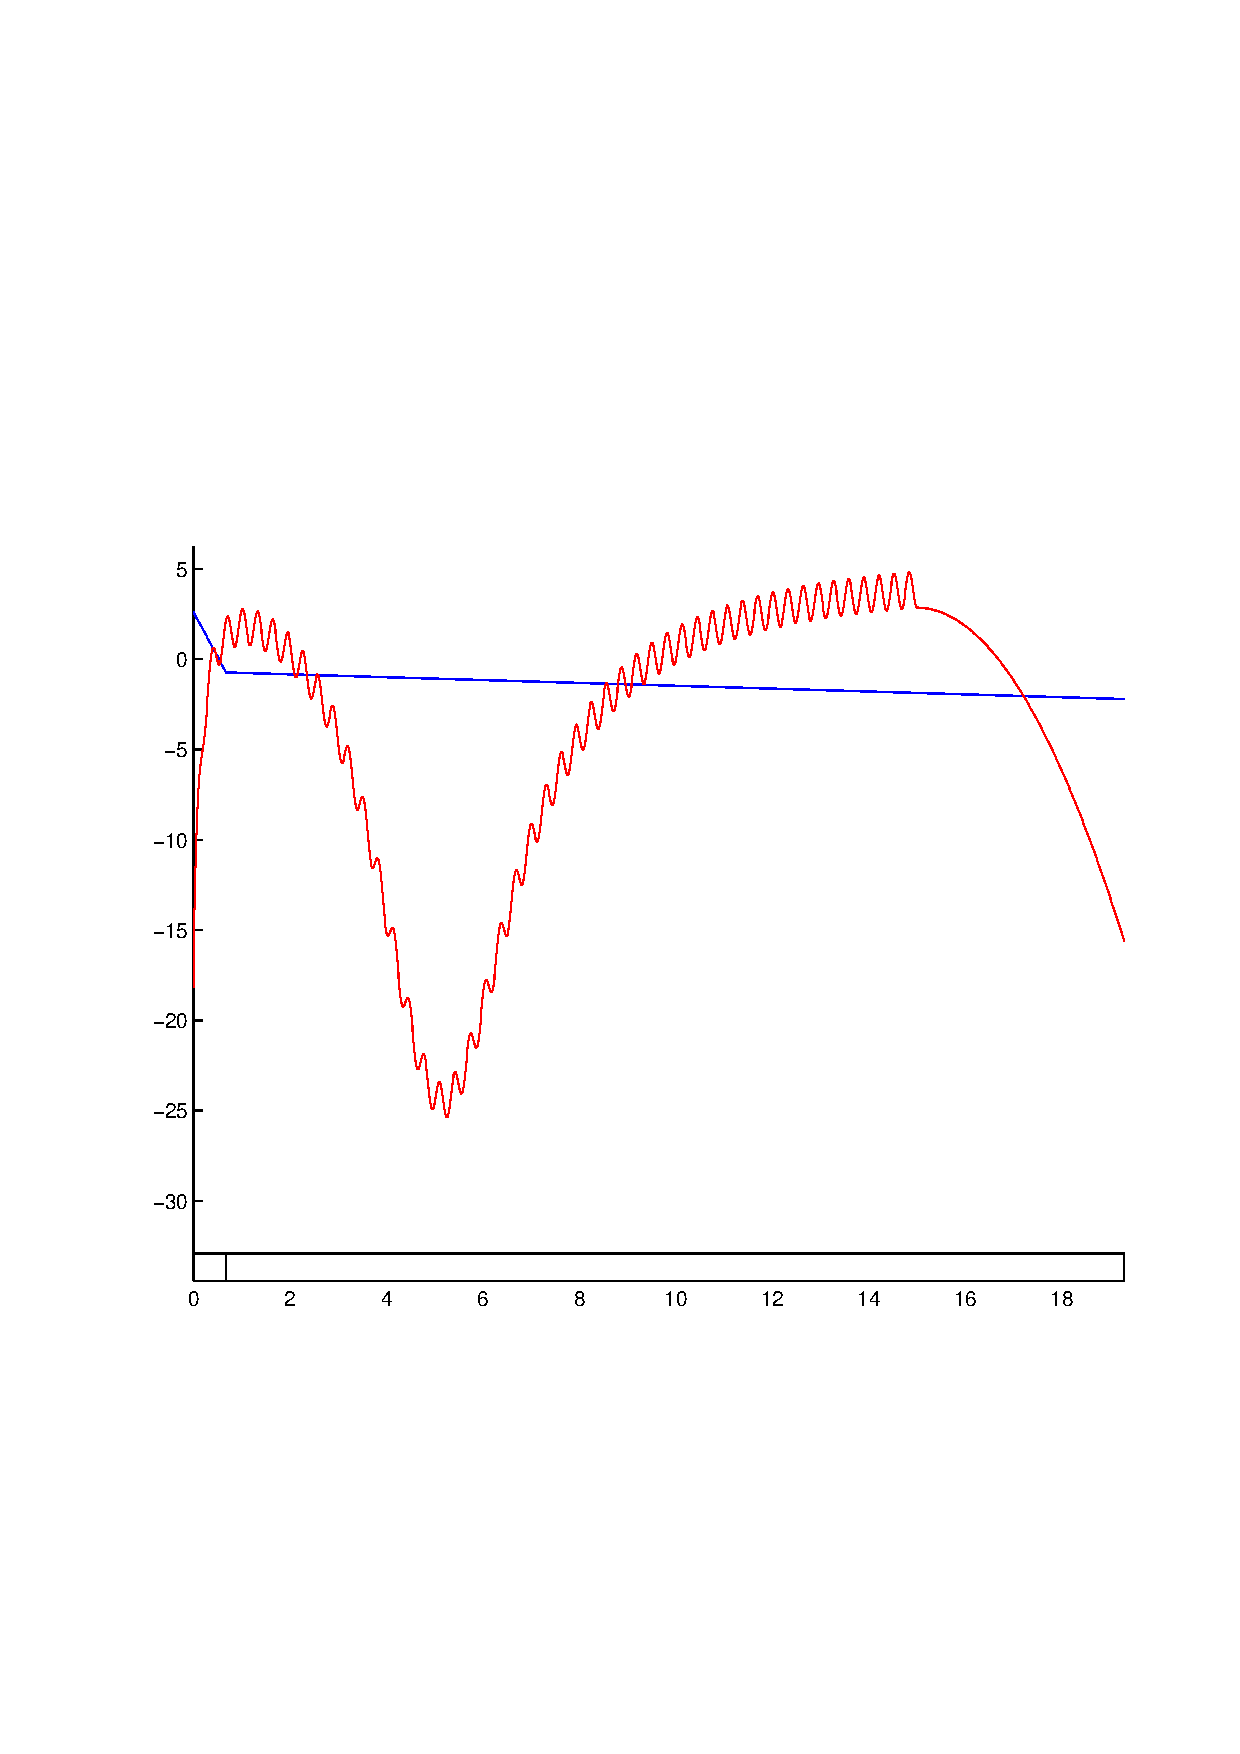
\includegraphics[width=0.3\textwidth]{Figure1}
%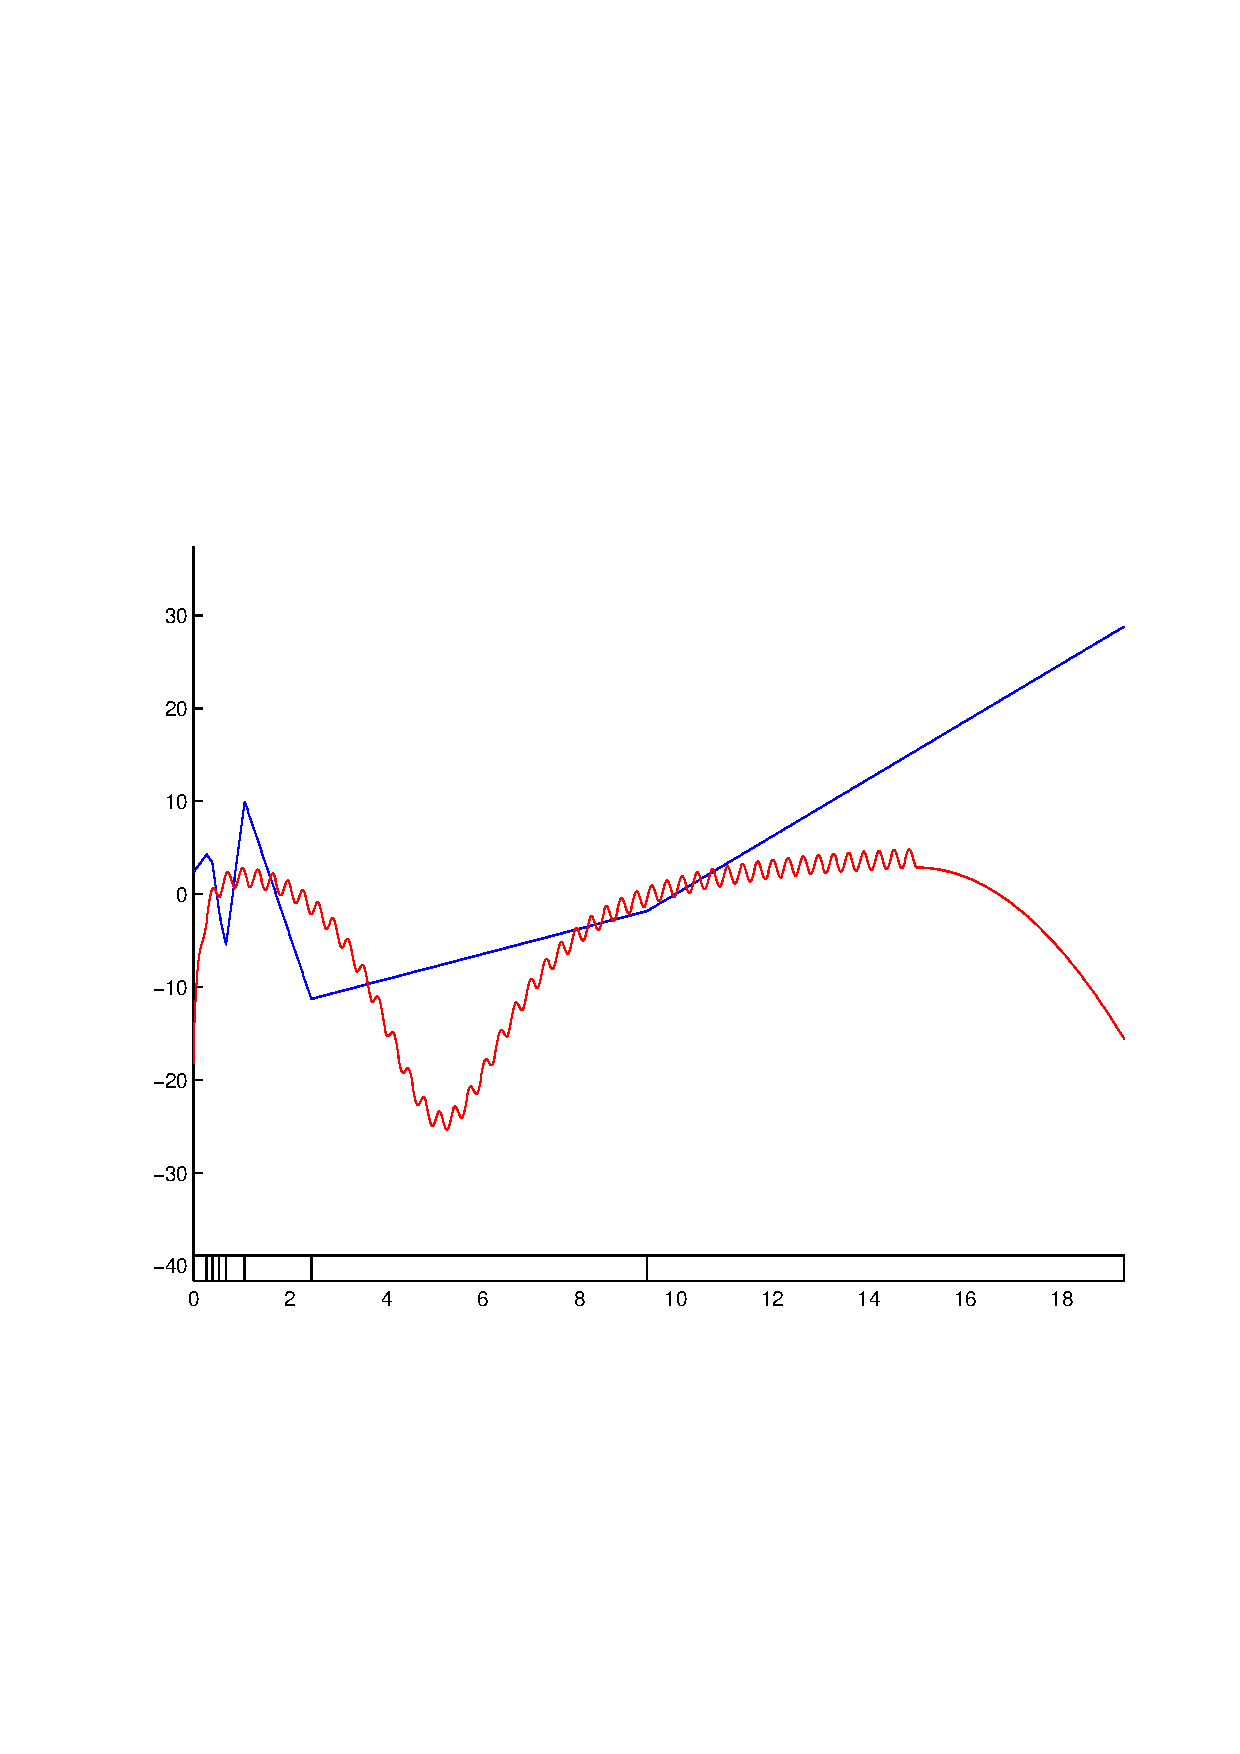
\includegraphics[width=0.3\textwidth]{Figure3}
%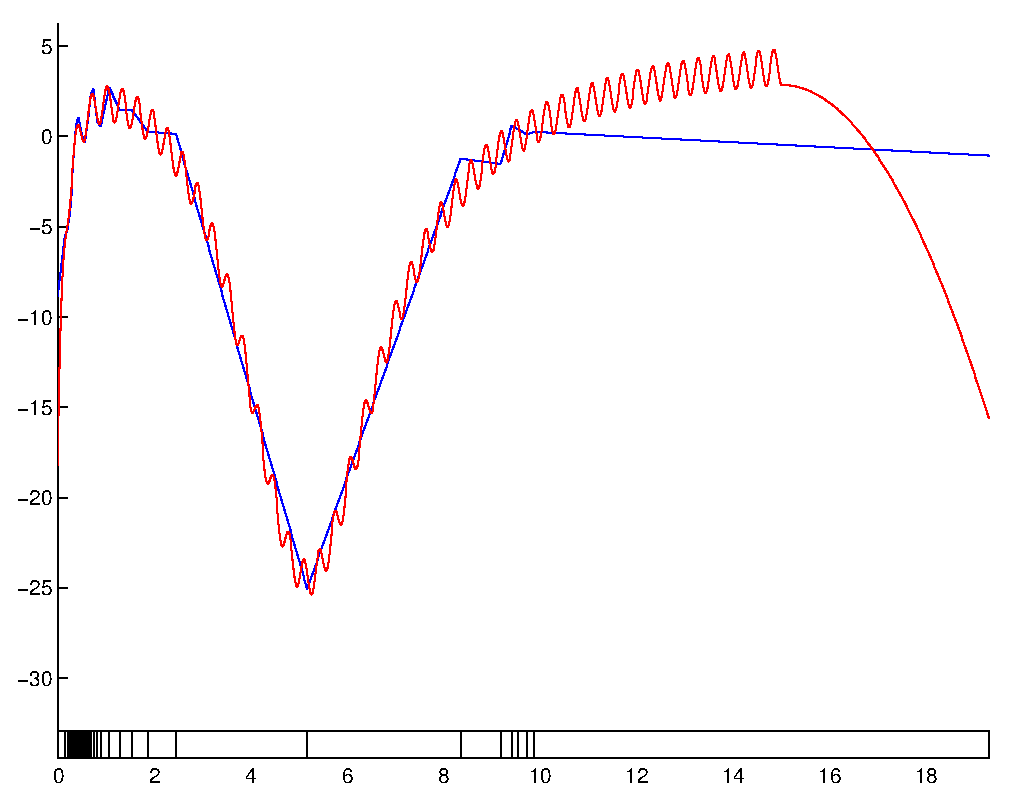
\includegraphics[width=0.3\textwidth]{Figure5}
%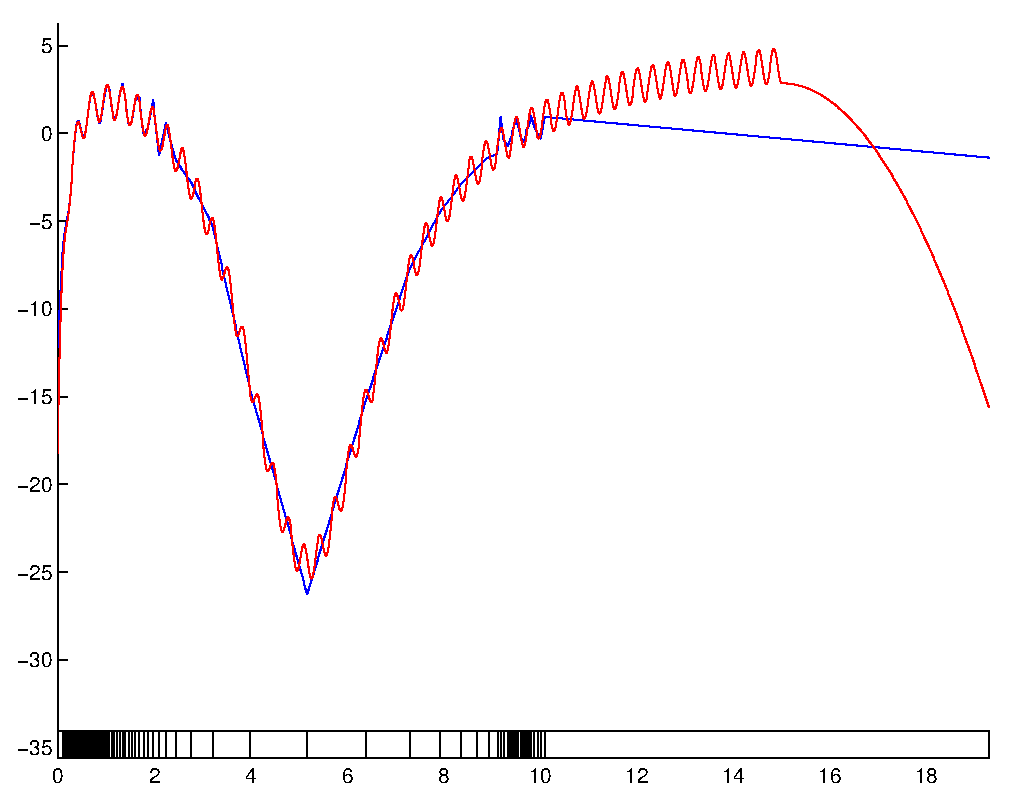
\includegraphics[width=0.3\textwidth]{Figure7}
%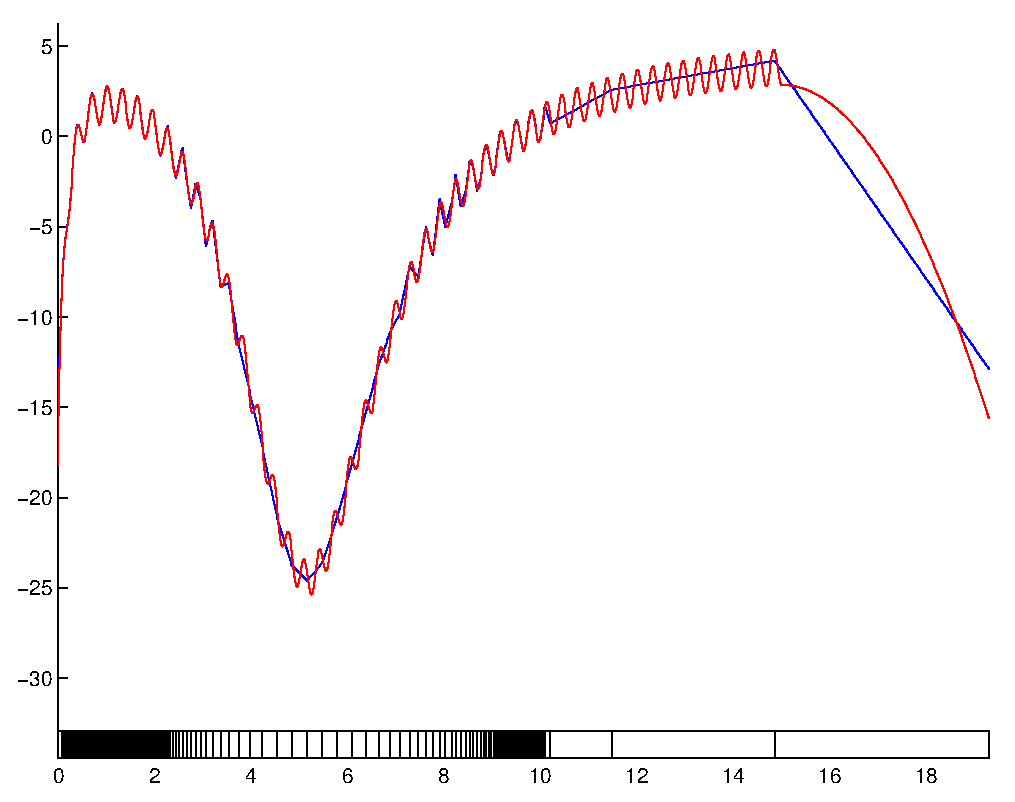
\includegraphics[width=0.3\textwidth]{Figure9}
%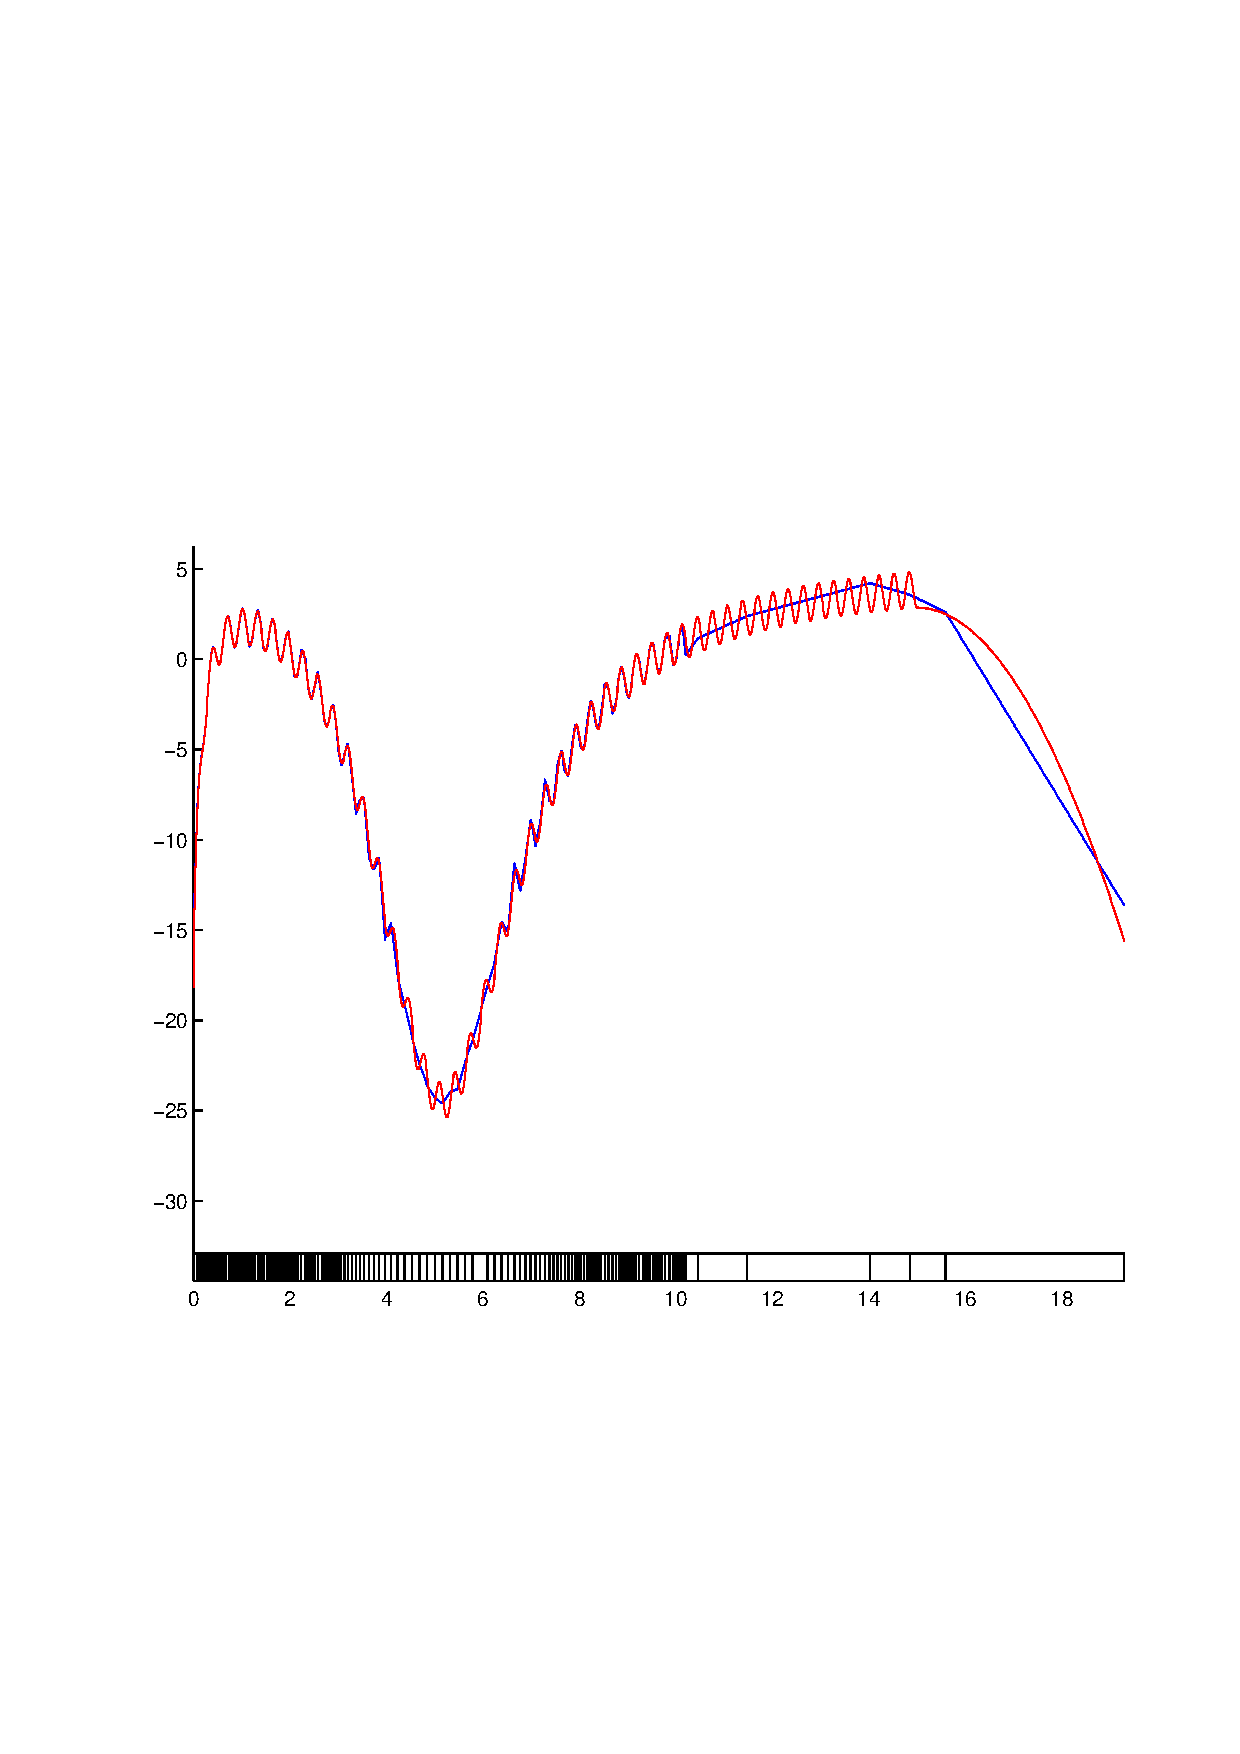
\includegraphics[width=0.3\textwidth]{Figure11} 
%\end{center}
%\caption{First preliminary numerical experiments indicating the successful recovery by an adaptive algorithm based on \eqref{fdproxy} of a potential function $a$ in a first order model of the type \eqref{fdgradientflow}. The potential $a$ to be recovered is displayed in red color and it's the strongly oscillating function. The blue function is the piecewise linear approximant computed at each successive iteration after adaptation of the underlying mesh, scketched on the bottom of the figures.}\label{firstnum}
%\end{figure}
%
%Despite the highly oscillatory nature of the parameter function $a$, the algorithm performs an excellent approximation, providing also a sort of "numerical homogenization" in those locations of the positive real line, where not enough data are provided by the evolution.

In this section we report several numerical experiments to document the validity and applicability of Theorem \ref{thm}. We will first show how the reconstruction of the unknown kernel $a$ gets better as the number of agents $N$ increases, in accordance with the $\Gamma$-convergence result reported in the last section. This feature holds true also for at least some interaction kernels not lying in the function space $X$, as shown in Figure \ref{variableN2}. We will then investigate empirically the validity of the coercivity condition \eqref{eq-coercive} comparing the functional $\mathcal E^{[a],N}(\widehat a_N)$ with $\|a - \widehat a_N\|_{L_2(\R_+,\rho^N)}^2$ where $\rho^N$ is constructed as $\rho$ but referring to the empirical measures $\mu^N$. Then we address  the behavior of $\mathcal E^{[a],N}(\widehat a_{N,M})$ for $N$ fixed, while we let the constraint constant  $M$ vary (here $\widehat a_{N,M}\equiv\widehat a_{N}$). Finally, we show how we can get a very satisfactory reconstruction of the unknown interaction kernel by keeping $N$ fixed and averaging the minimizers of the functional $\mathcal E^{[a],N}$ obtained from several samples of the initial data distribution $\mu_0$.

\subsection{Numerical framework}\label{numfram}

All experiments  rely on a common numerical set-up, which we clarify in this section. All the initial data $\mu^N_0$ are drawn from a common probability distribution $\mu_0$ which is the uniform distribution on the $d$-dimensional cube $[-L,L]^d$. For every $\mu^N_0$, we simulate the evolution of the system starting from $\mu^N_0$ until time $T$, and we shall denote with $R$ the maximal distance between particles reached during the time frame $[0,T]$. Notice that we have at our disposal only a finite sequence of snapshots of the dynamics: if we denote with $0 = t_0 < t_1 < \ldots < t_m = T$ the time instants at which these snapshots are taken, we can consider the \textit{discrete-time error functional}
\begin{align*}
\mathcal{E}^{[a],N}_\Delta(\widehat{a}) & = \frac{1}{m} \sum^m_{k = 1} \frac{1}{N} \sum^N_{j = 1} \left| \frac{1}{N} \sum^N_{i = 1} \widehat{a}(|x_j(t_k) - x_i(t_k)|)(x_j(t_k) - x_i(t_k)) - \dot{x}_i(t_k)\right|^2,
\end{align*}
which is the time-discrete counterpart of the continuous-time error functional $\mathcal{E}^{[a],N}$. As already mentioned in the introduction, derivatives $\dot{x}_i(t_k)$ appearing in $\mathcal{E}^{[a],N}_\Delta$ are actually approximated as well by finite differences: in our experiments we will use the simplest approximation
\begin{align*}
\dot{x}_i(t_k) = \frac{x_i(t_k) - x_i(t_{k-1})}{t_k - t_{k-1}}, \text{ for every } k \geq 1.
\end{align*}

Regarding the reconstruction procedure, we fix the constraint level $M>0$ and consider the sequence of invading subspaces $V_N$ of $X_{M,K}$ ($K=[0,2 R]$ here) generated by a B-spline basis with $D(N) $ elements supported on $[0,2 R]$: for every element $\widehat{a} \in V_N$ it holds
\begin{align*}
	\widehat{a}(r) = \sum^{D(N)}_{\lambda = 1} a_{\lambda} \varphi_{\lambda}(r), \qquad r \in [0,2R].
\end{align*}
In order for $V_N$ to increase in $N$ and invade $X_{M,K}$, we let $D(N)$ be a strictly increasing function of $N$. For the sake of simplicity, we shall employ a \textit{linear uniform} B-spline basis supported on the interval $[0,2 R]$ with $0$-smoothness conditions at the boundary, see \cite{deboor}.
%To avoid the inconvenience of having a reconstructed kernel with value at $0$ and at $R$ equal to $0$, we consider the knots of the B-spline basis to be
%\begin{align*}
%\left[0,0,0,\frac{R}{(D(N)-2)},\ldots,\frac{(D(N) - 3)R}{(D(N)-2)},R,R,R\right].
%\end{align*}
%\MFcomment{Non capisco questa cosa della spline con discontinuit\`a! Mi pare che i nodi sopra menzionati si riferiscano
%solo all'estremo $R$. E in $0$? Se non si riesce a spiegare bene che si sta facendo qui \`e meglio togliere questi dettagli.}
%i.e., the spline reconstruction has in $0$ and $R$ two discontinuity points.

Whenever $\widehat{a} \in V_N$, we can rewrite the functional $\mathcal{E}^{[a],N}_\Delta$ as
\begin{align*}
\mathcal{E}^{[a],N}_\Delta(\widehat{a}) & = \frac{1}{m} \sum^m_{k = 1} \frac{1}{N} \sum^N_{j = 1} \left| \frac{1}{N} \sum^N_{i = 1} \sum^{D(N)}_{\lambda = 1} a_{\lambda} \varphi_{\lambda}(|x_j(t_k) - x_i(t_k)|)(x_j(t_k) - x_i(t_k)) - \dot{x}_i(t_k)\right|^2 \\
& = \frac{1}{m} \sum^m_{k = 1} \frac{1}{N} \sum^N_{j = 1} \left| \sum^{D(N)}_{\lambda = 1} a_{\lambda} \frac{1}{N} \sum^N_{i = 1} \varphi_{\lambda}(|x_j(t_k) - x_i(t_k)|)(x_j(t_k) - x_i(t_k)) - \dot{x}_i(t_k)\right|^2 \\
& = \frac{1}{mN} \left\| \mathbf C  \vec{a} - \vec v \right\|^2_{2},
\end{align*}
where $\vec{a} = (a_1, \ldots, a_{D(N)})$, $\vec v = (\dot{x}_1(t_1), \ldots, \dot{x}_N(t_1), \ldots,\dot{x}_1(t_m), \ldots, \dot{x}_N(t_m))$ and the tensor $\mathbf C \in \R^{d\times Nm \times D(N)}$ satisfies for every $j = 1, \ldots,N$, $k = 1, \ldots,m$, $\lambda = 1, \ldots,D(N)$
\begin{align*}
\mathbf C(jk,\lambda) = \frac{1}{N} \sum^N_{i = 1} \varphi_{\lambda}(|x_j(t_k) - x_i(t_k)|)(x_j(t_k) - x_i(t_k)) \in \R^d.
\end{align*}

We shall numerically implement the constrained minimization with the software CVX \cite{cvx,gb08}, which allows constraints and objectives to be specified using standard MATLAB expression syntax. In order to use it, we need to rewrite the constraint of our minimization problem, which reads
\begin{align*}
	\|a\|_{L_{\infty}([0,R])} + \|a'\|_{L_{\infty}([0,R])} \leq M,
\end{align*}
using only the minimization variable of the problem, which is the vector of coefficients of the B-spline basis $\vec{a}$. Notice that the property of being a linear B-spline basis implies that, for every $\lambda = 1, \ldots, D(N)-1$, the property $\supp(\varphi_{\lambda}) \cap \supp(\varphi_{\lambda + j}) \not= \emptyset$ holds if and only if $j = 1$. Hence, for every $a \in V_N$ we have
\begin{align*}
\|a\|_{L_{\infty}([0,2 R])} &= \max_{r \in [0,R]} \left|\sum^{D(N)}_{\lambda = 1} a_{\lambda} \varphi_{\lambda}(r)\right|
% \leq \max_{r \in [0,2 R]} \sum^{D(N)}_{\lambda = 1} \left|a_{\lambda} \varphi_{\lambda}(r)\right| 
 \leq \max_{\lambda = 1, \ldots, D(N)-1} \left(|a_{\lambda}| + |a_{\lambda+1}|\right) 
 \leq 2 \|\vec{a}\|_{\infty},
\end{align*}
\begin{align*}
\|a'\|_{L_{\infty}([0,2 R])} &= \max_{r \in [0,2 R]} \left|\sum^{D(N)}_{\lambda = 1} a_{\lambda} \varphi'_{\lambda}(r)\right| 
 \leq \max_{\lambda = 1, \ldots, D(N)-1} |a_{\lambda+1} - a_{\lambda}|
 = \|\mathbf D\vec{a}\|_{\infty},
\end{align*}
where, in the last line, $\mathbf  D$ is the standard finite difference matrix
\begin{align*}
\mathbf  D = \begin{bmatrix}
    1       & -1 & 0 & \dots & 0 & 0 \\
    0     & 1 & -1 & \dots & 0 & 0 \\
   \vdots & \vdots & \ddots & \ddots & \vdots & \vdots \\ \\
    0       & 0 & 0 & \dots & 1 & -1 \\
    0       & 0 & 0 & \dots & 0 & 0
\end{bmatrix}.
\end{align*}
We therefore replace the constrained minimization problem
\begin{align*}
\min_{\widehat{a} \in V_N} \mathcal{E}^{[a],N}(\widehat{a}) \quad \text{ subject to } \quad \|\widehat{a}\|_{L_{\infty}([0,R])} + \|\widehat{a}'\|_{L_{\infty}([0,R])} \leq M,
\end{align*}
by
\begin{align}\label{problem2}
\min_{\vec{a} \in \R^{D(N)}} \frac{1}{mN} \left\|\mathbf C \vec{a} - \vec v \right\|^2_{2} \quad \text{ subject to } \quad 2\|\vec{a}\|_{\infty} + \|\mathbf D\vec{a}\|_{\infty} \leq M\,,
\end{align}
which has weaker constraints, but is amenable to numerical solution.
The byproduct of the time discretization and the reformulation of the constraint is that minimizers of problem \eqref{problem2} may not be precisely the minimizers of the original one. This is the price to pay for this simple numerical implementation of the $L_\infty$-constraints. Despite such a crude discrete model,  we still observe all the approximation properties proved in the previous sections and the implementation results both simple and effective.

\subsection{Varying $N$}

In Figure \ref{variableN} we show the reconstruction of a truncated Lennard-Jones type interaction kernel obtained with different values of $N$. Table \ref{tab:fig1} reports the values of the different parameters.

\begin{table}[h!]% \label{Table1}
\begin{center}
\begin{tabular}{ |c|c|c|c|c|c| }
\hline
  $d$ & $L$ & $T$ & $M$ & $N$ & $D(N)$ \\
\hline
\hline
  $2$ & $3$ & $0.5$ & $100$ & $[10,20,40,80]$ & $2N$ \\
\hline
\end{tabular}
\end{center}
\vspace{-0.5cm}
\caption{Parameter values for Figure \ref{variableN} and Figure \ref{variableN2}.} \label{tab:fig1} 
\end{table}

It is clearly visible how the the piecewise linear approximant (displayed in blue) gets closer and closer to the potential to be recovered (in red), as predicted by the theoretical results of the previous sections. What is however surprising is that the same behavior is witnessed in Figure \ref{variableN2}, where the algorithm is applied to an interaction kernel $a$ not belonging to the function space $X$ (due to its singularity at the origin) with the same specifications reported in Table \ref{tab:fig1}. In particular, the algorithm performs an excellent approximation despite the highly oscillatory nature of the function $a$ and produce a natural numerical homogeneization when the discretization is not fine enough.

\begin{figure}[h!]
\begin{center}
\hspace{-0.7cm}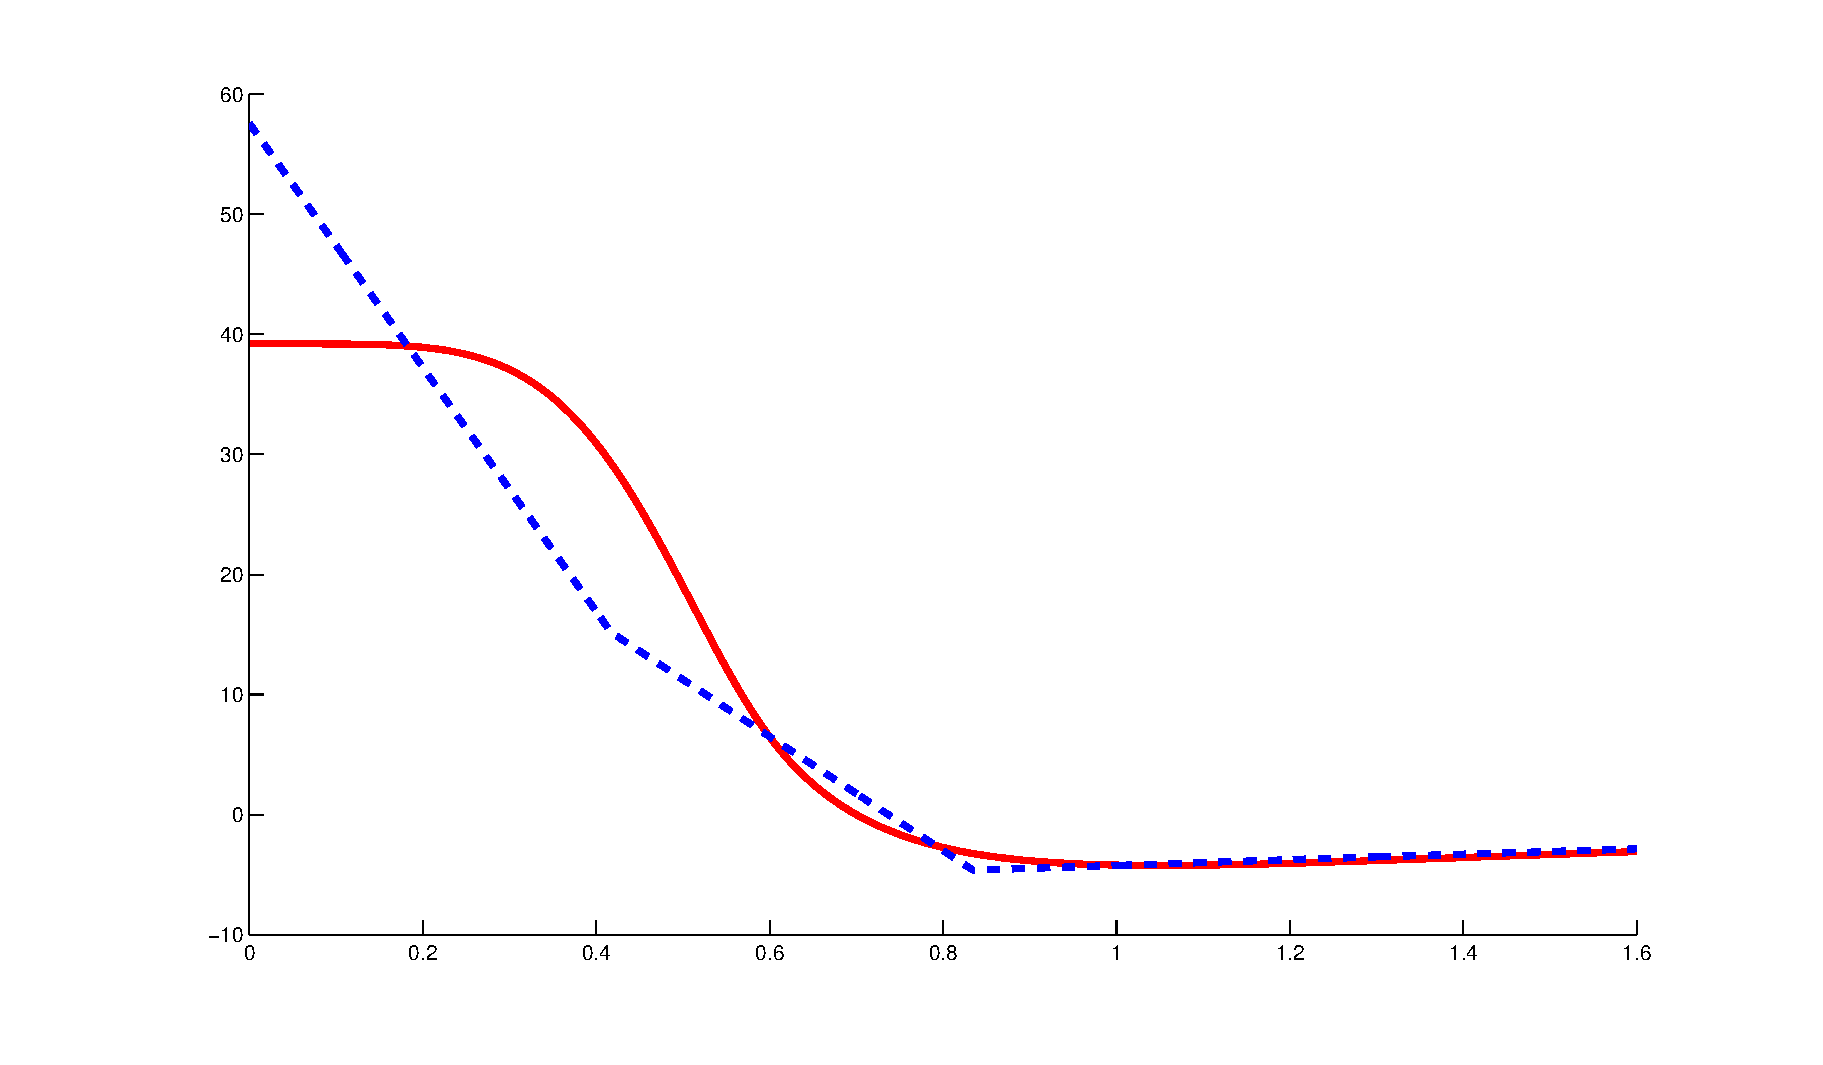
\includegraphics[width=0.55\textwidth]{figfun810agents}\hspace{-0.9cm}
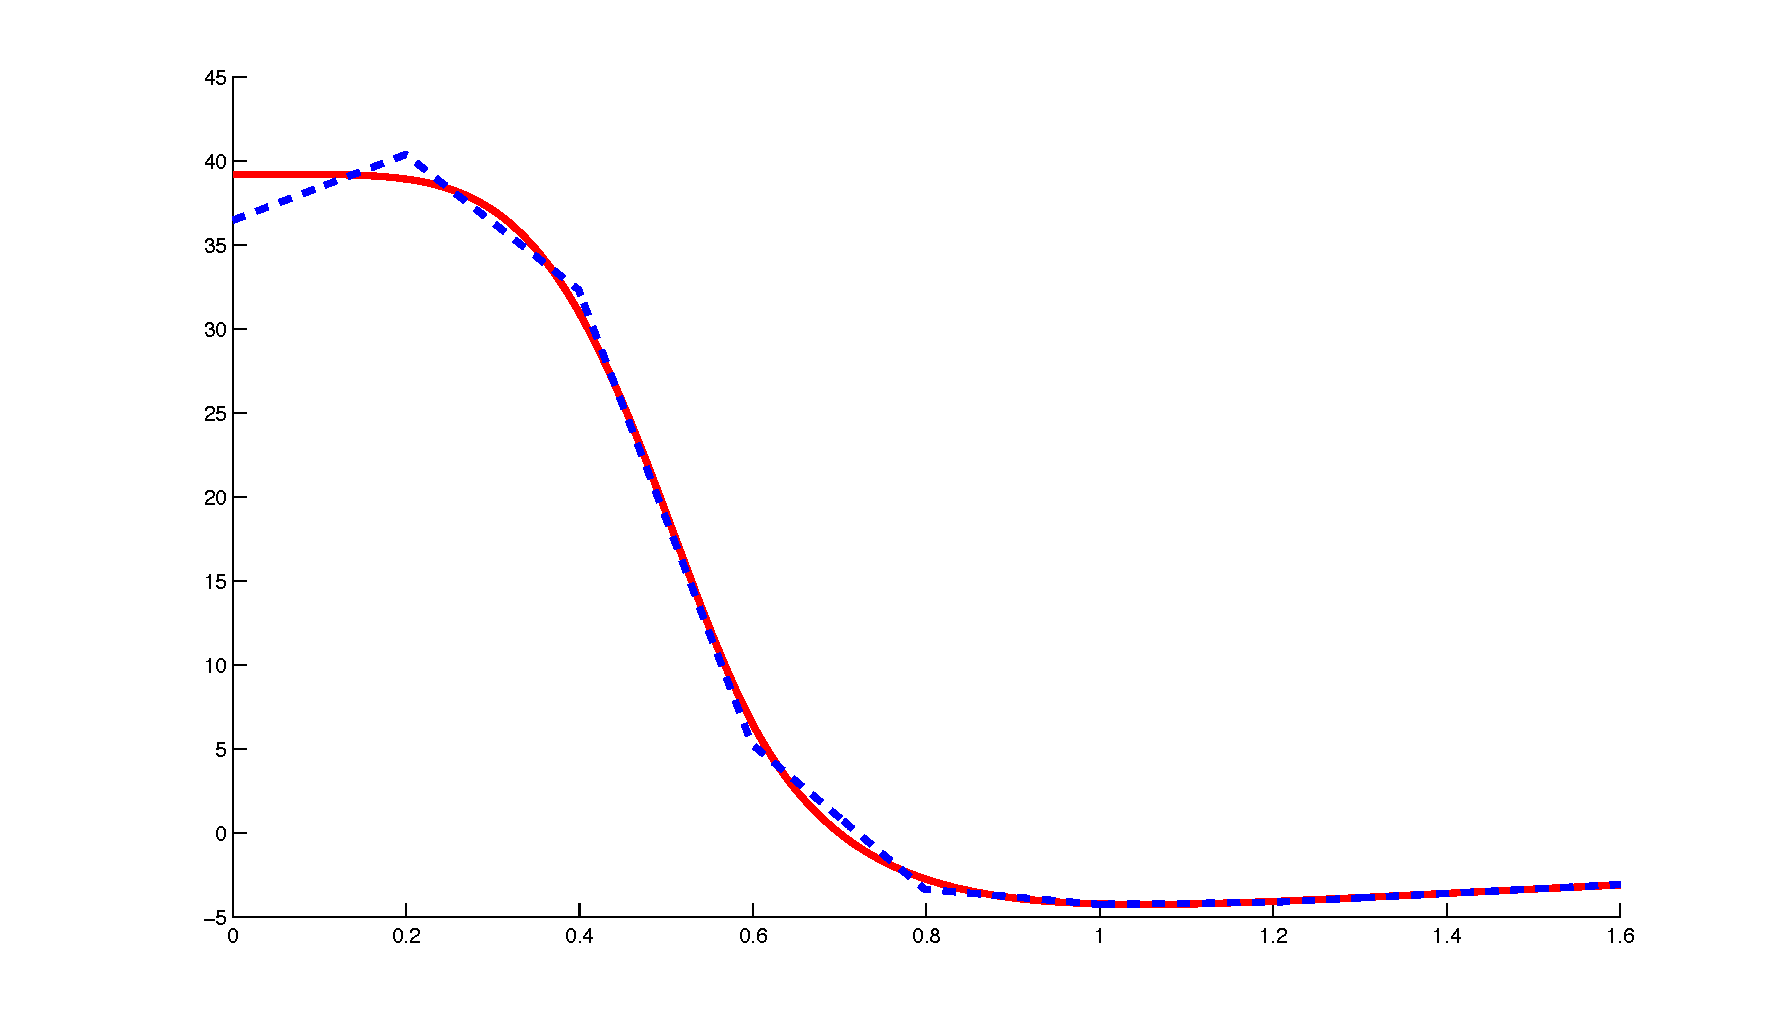
\includegraphics[width=0.55\textwidth]{figfun820agents}\\
\hspace{-0.7cm}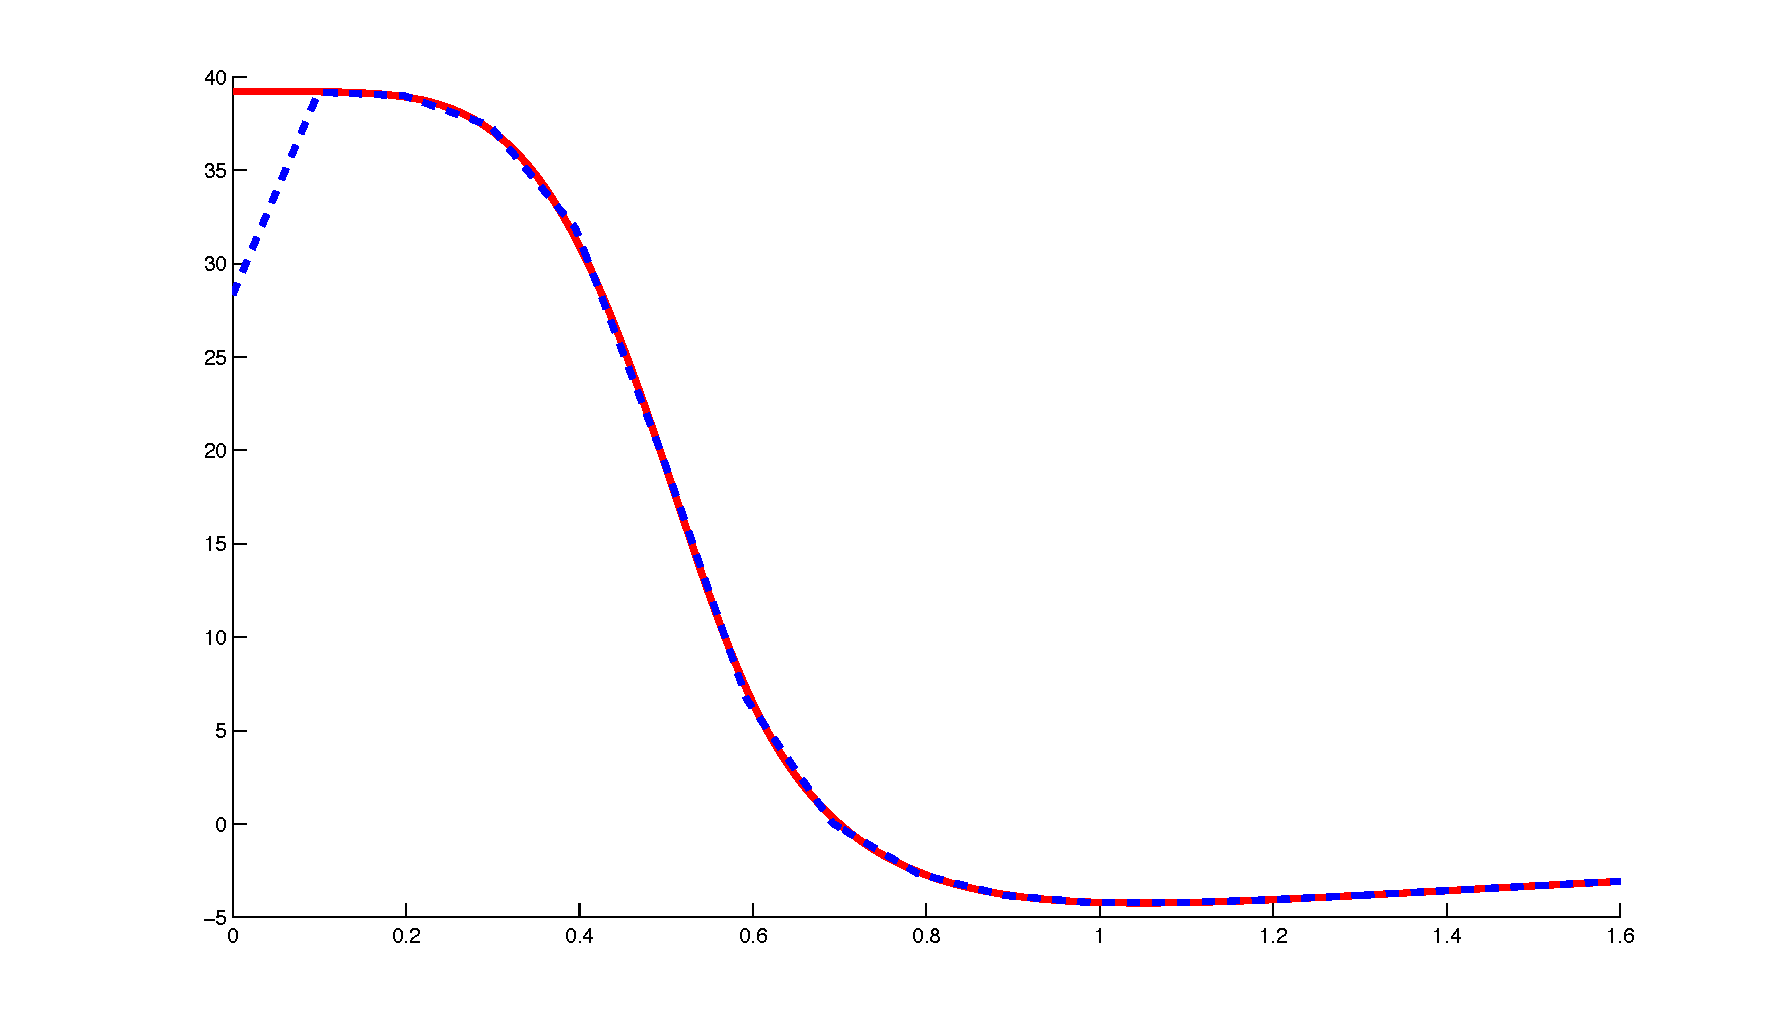
\includegraphics[width=0.55\textwidth]{figfun840agents}\hspace{-0.9cm}
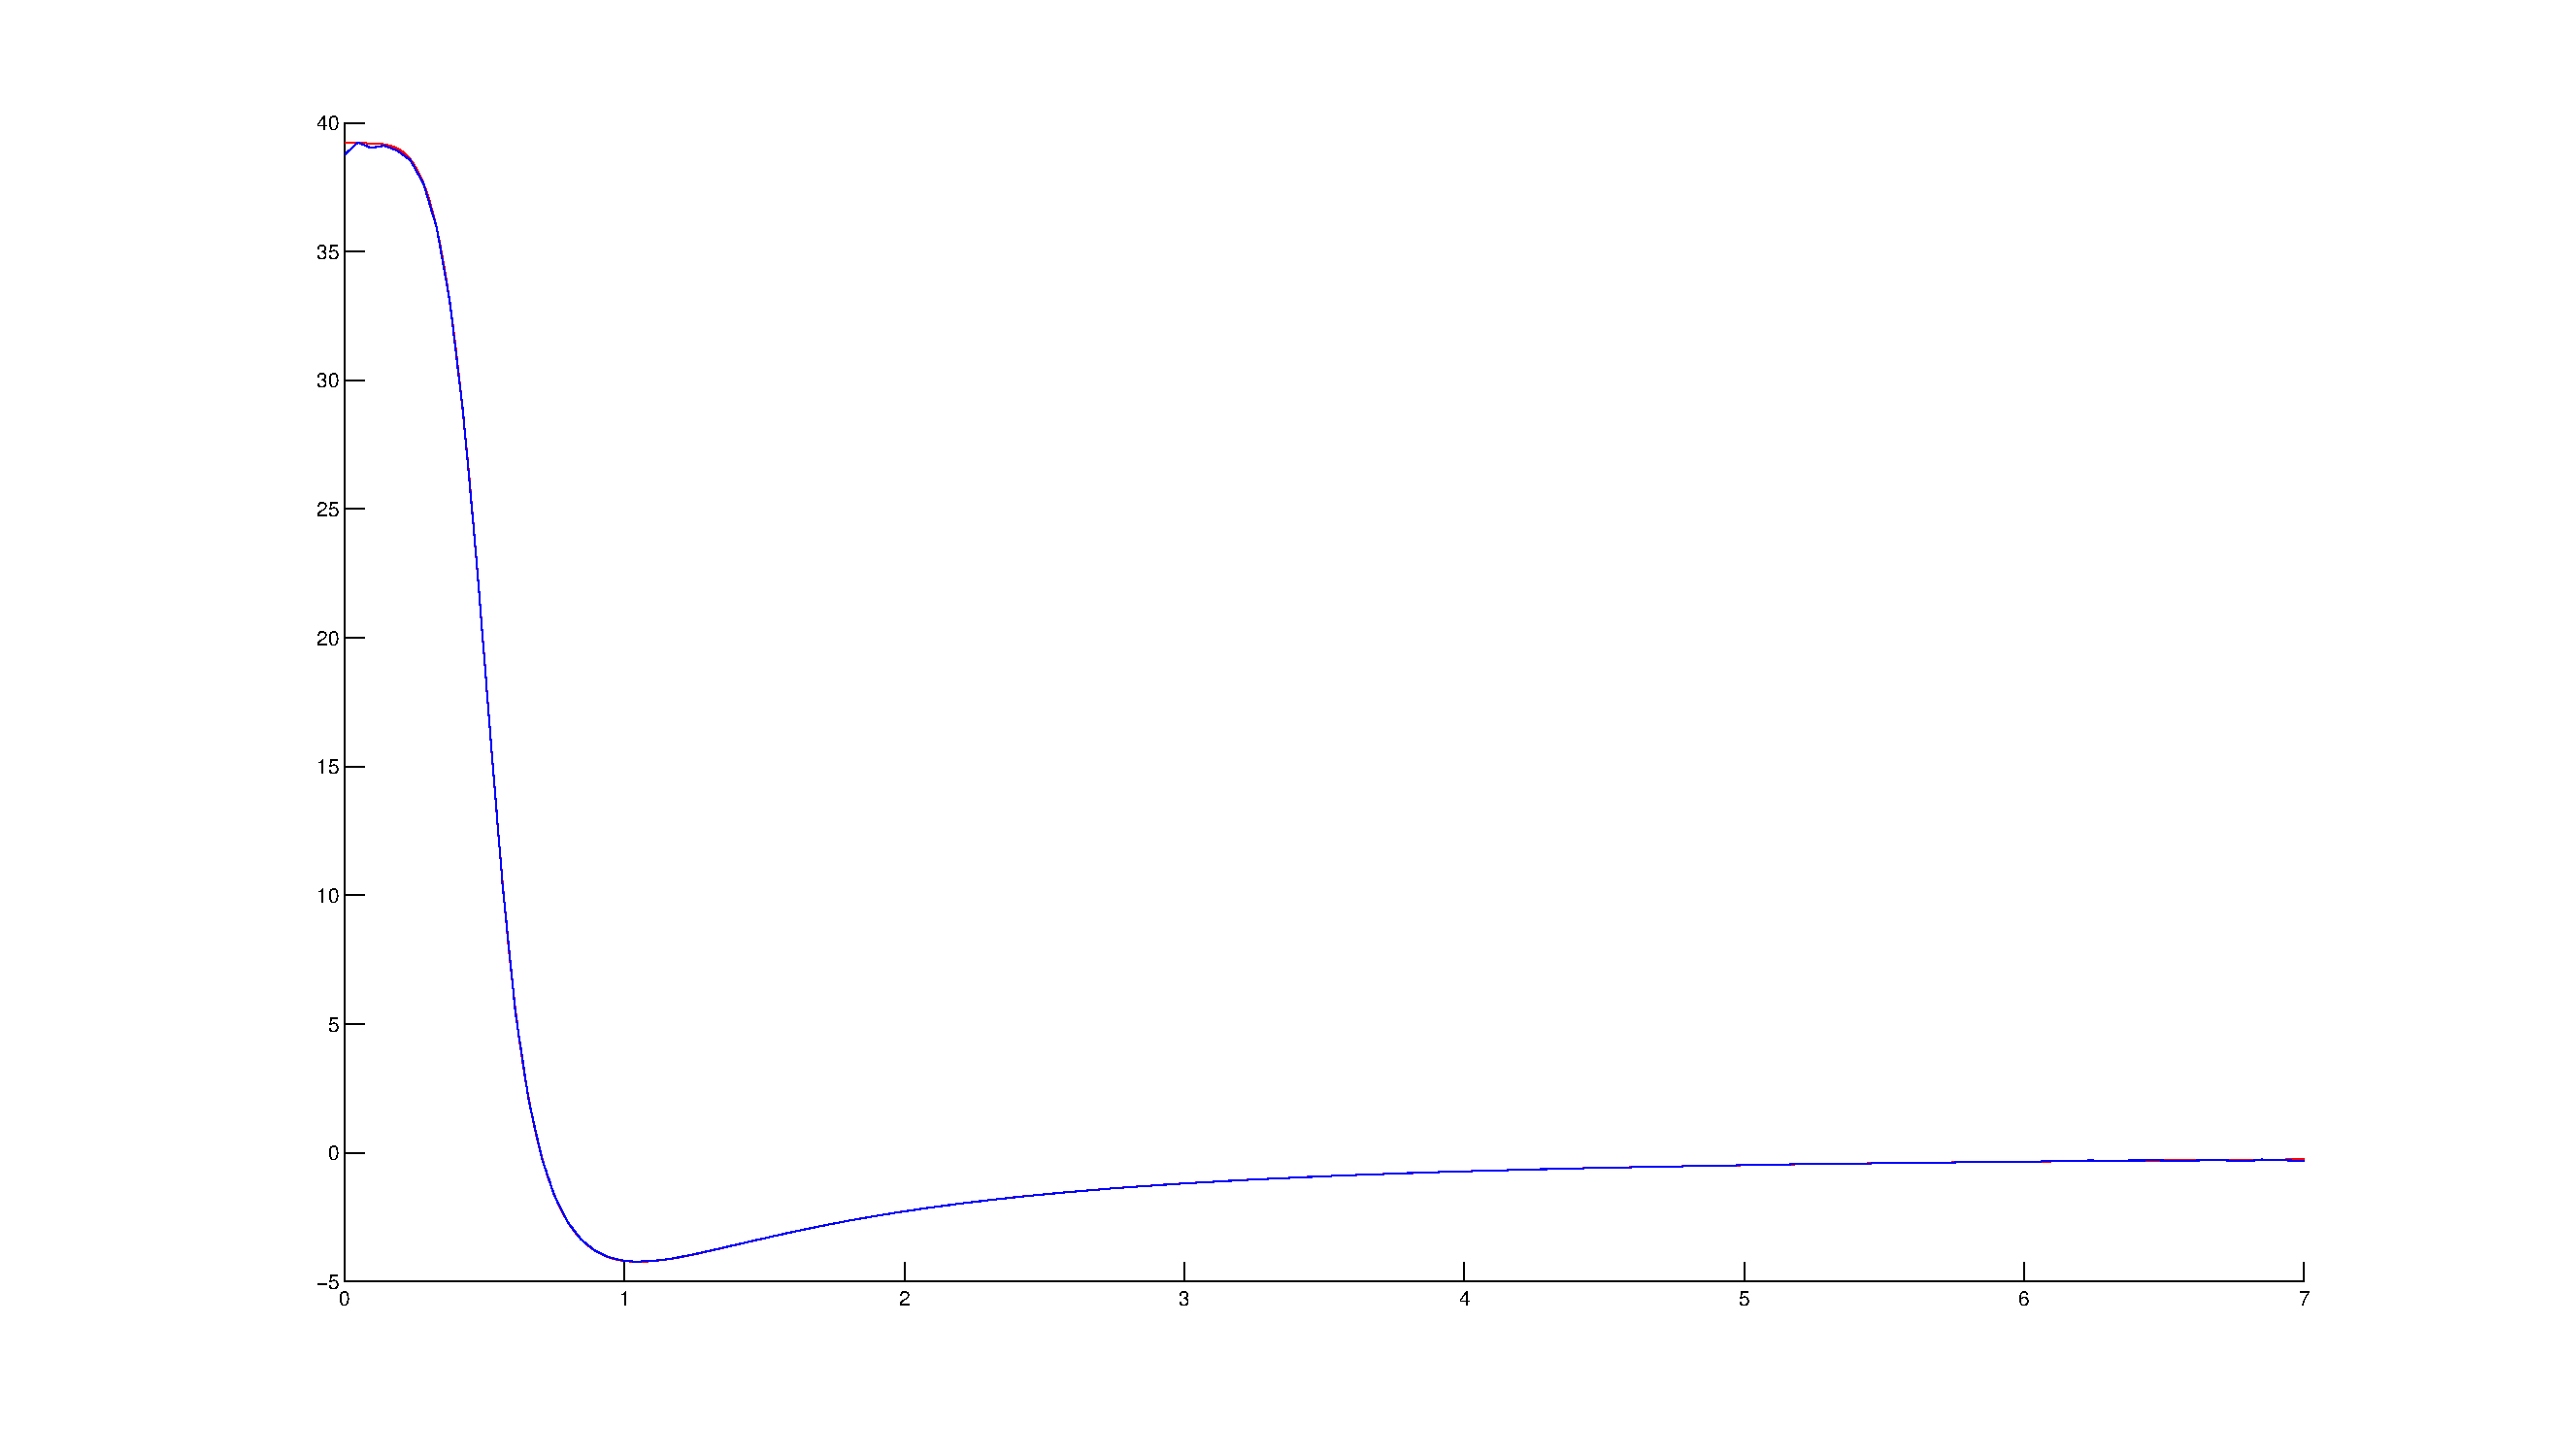
\includegraphics[width=0.55\textwidth]{figfun880agents}
\end{center}
\caption{Iterative reconstruction of a potential with different values of $N$. In red: the unknown kernel. In blue: its reconstruction by minimization of $\mathcal{E}^{[a],N}$. From left-top to right-bottom: reconstruction with $N = 10, 20, 40, 80$ agents. We notice that the convergence at $0$ is slower in view of the quadratic polynomical weight $s^2$ as in \eqref{rho}, for which less information actually is available around $0$.}\label{variableN}
\end{figure}

\begin{figure}[h!]
\begin{center}
\hspace{-0.7cm}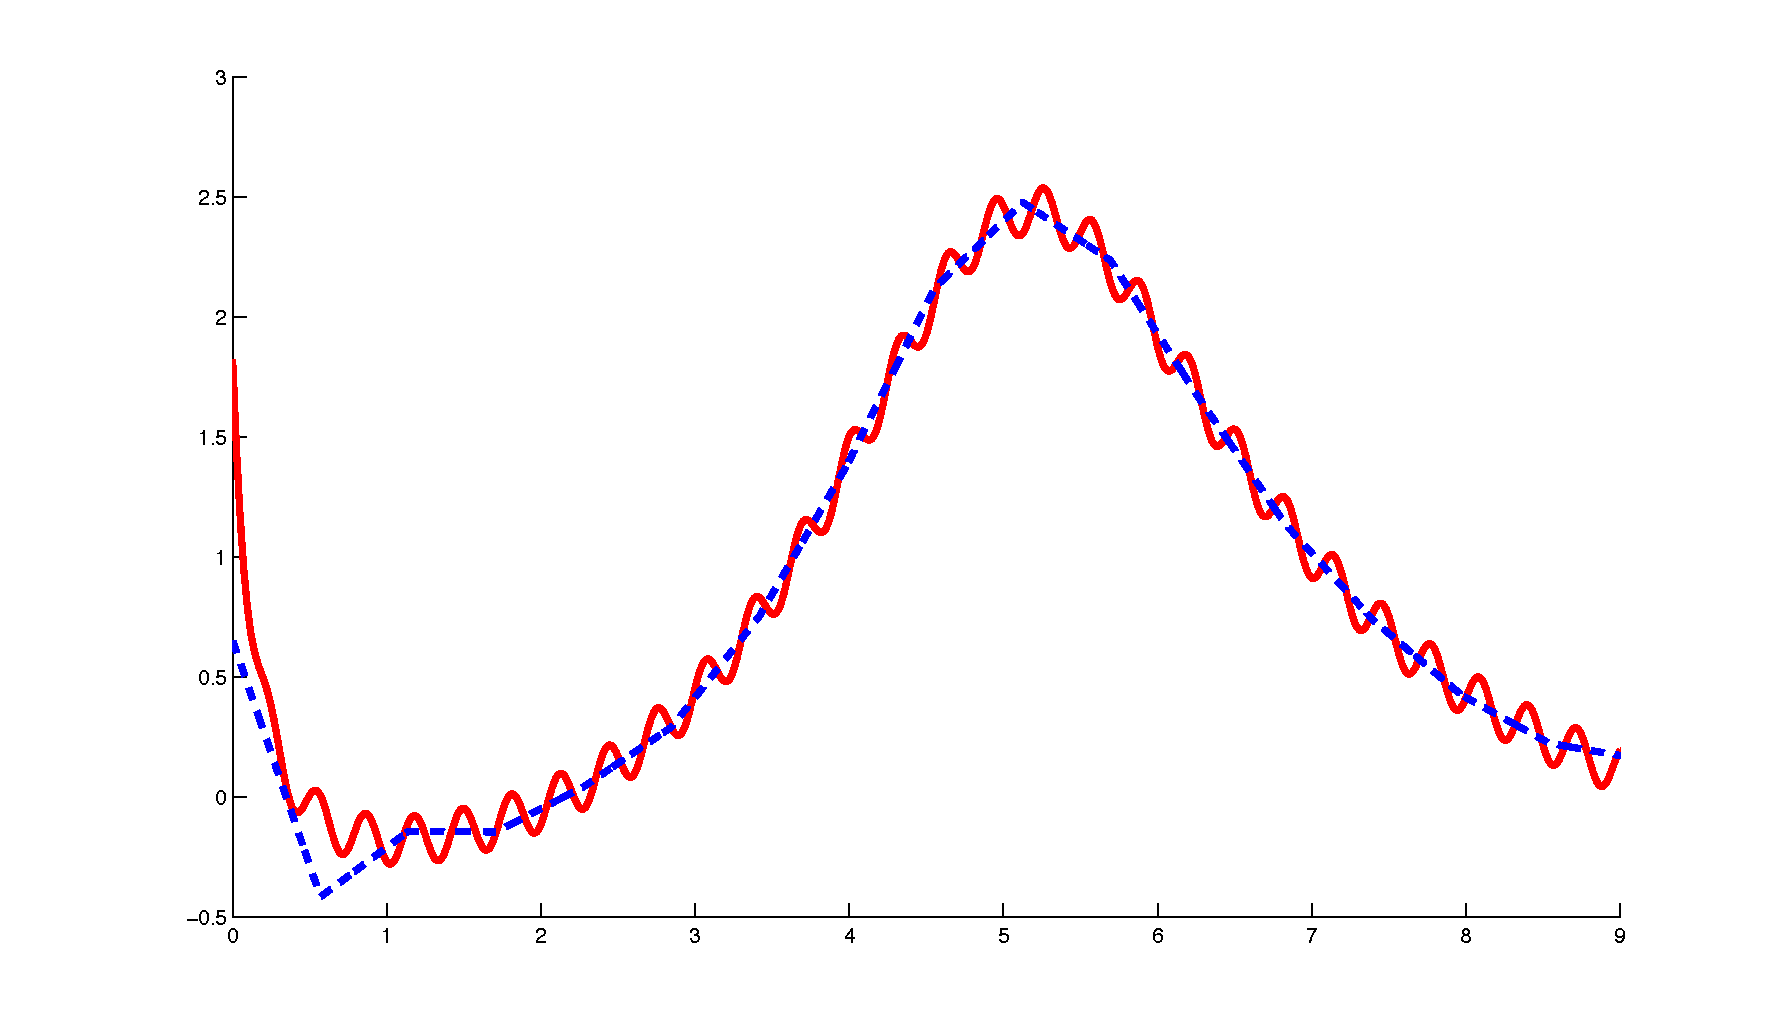
\includegraphics[width=0.55\textwidth]{figfun610agents}\hspace{-0.9cm}
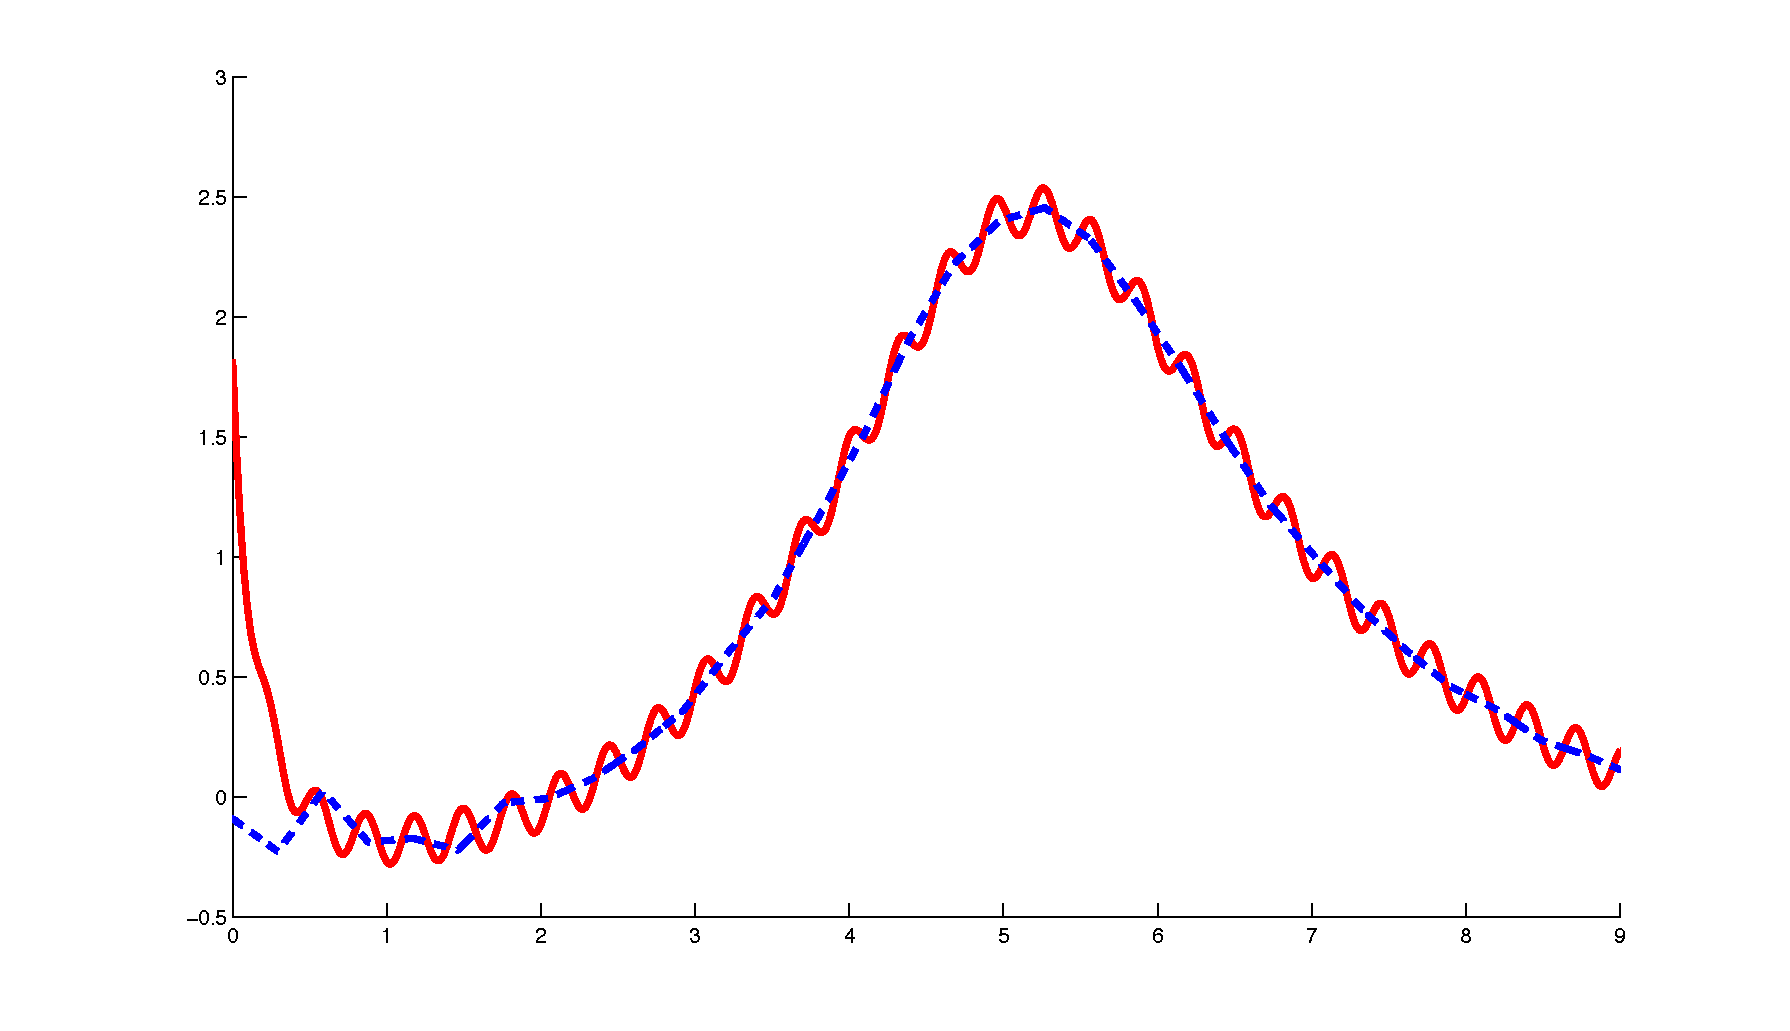
\includegraphics[width=0.55\textwidth]{figfun620agents}\\
\hspace{-0.7cm}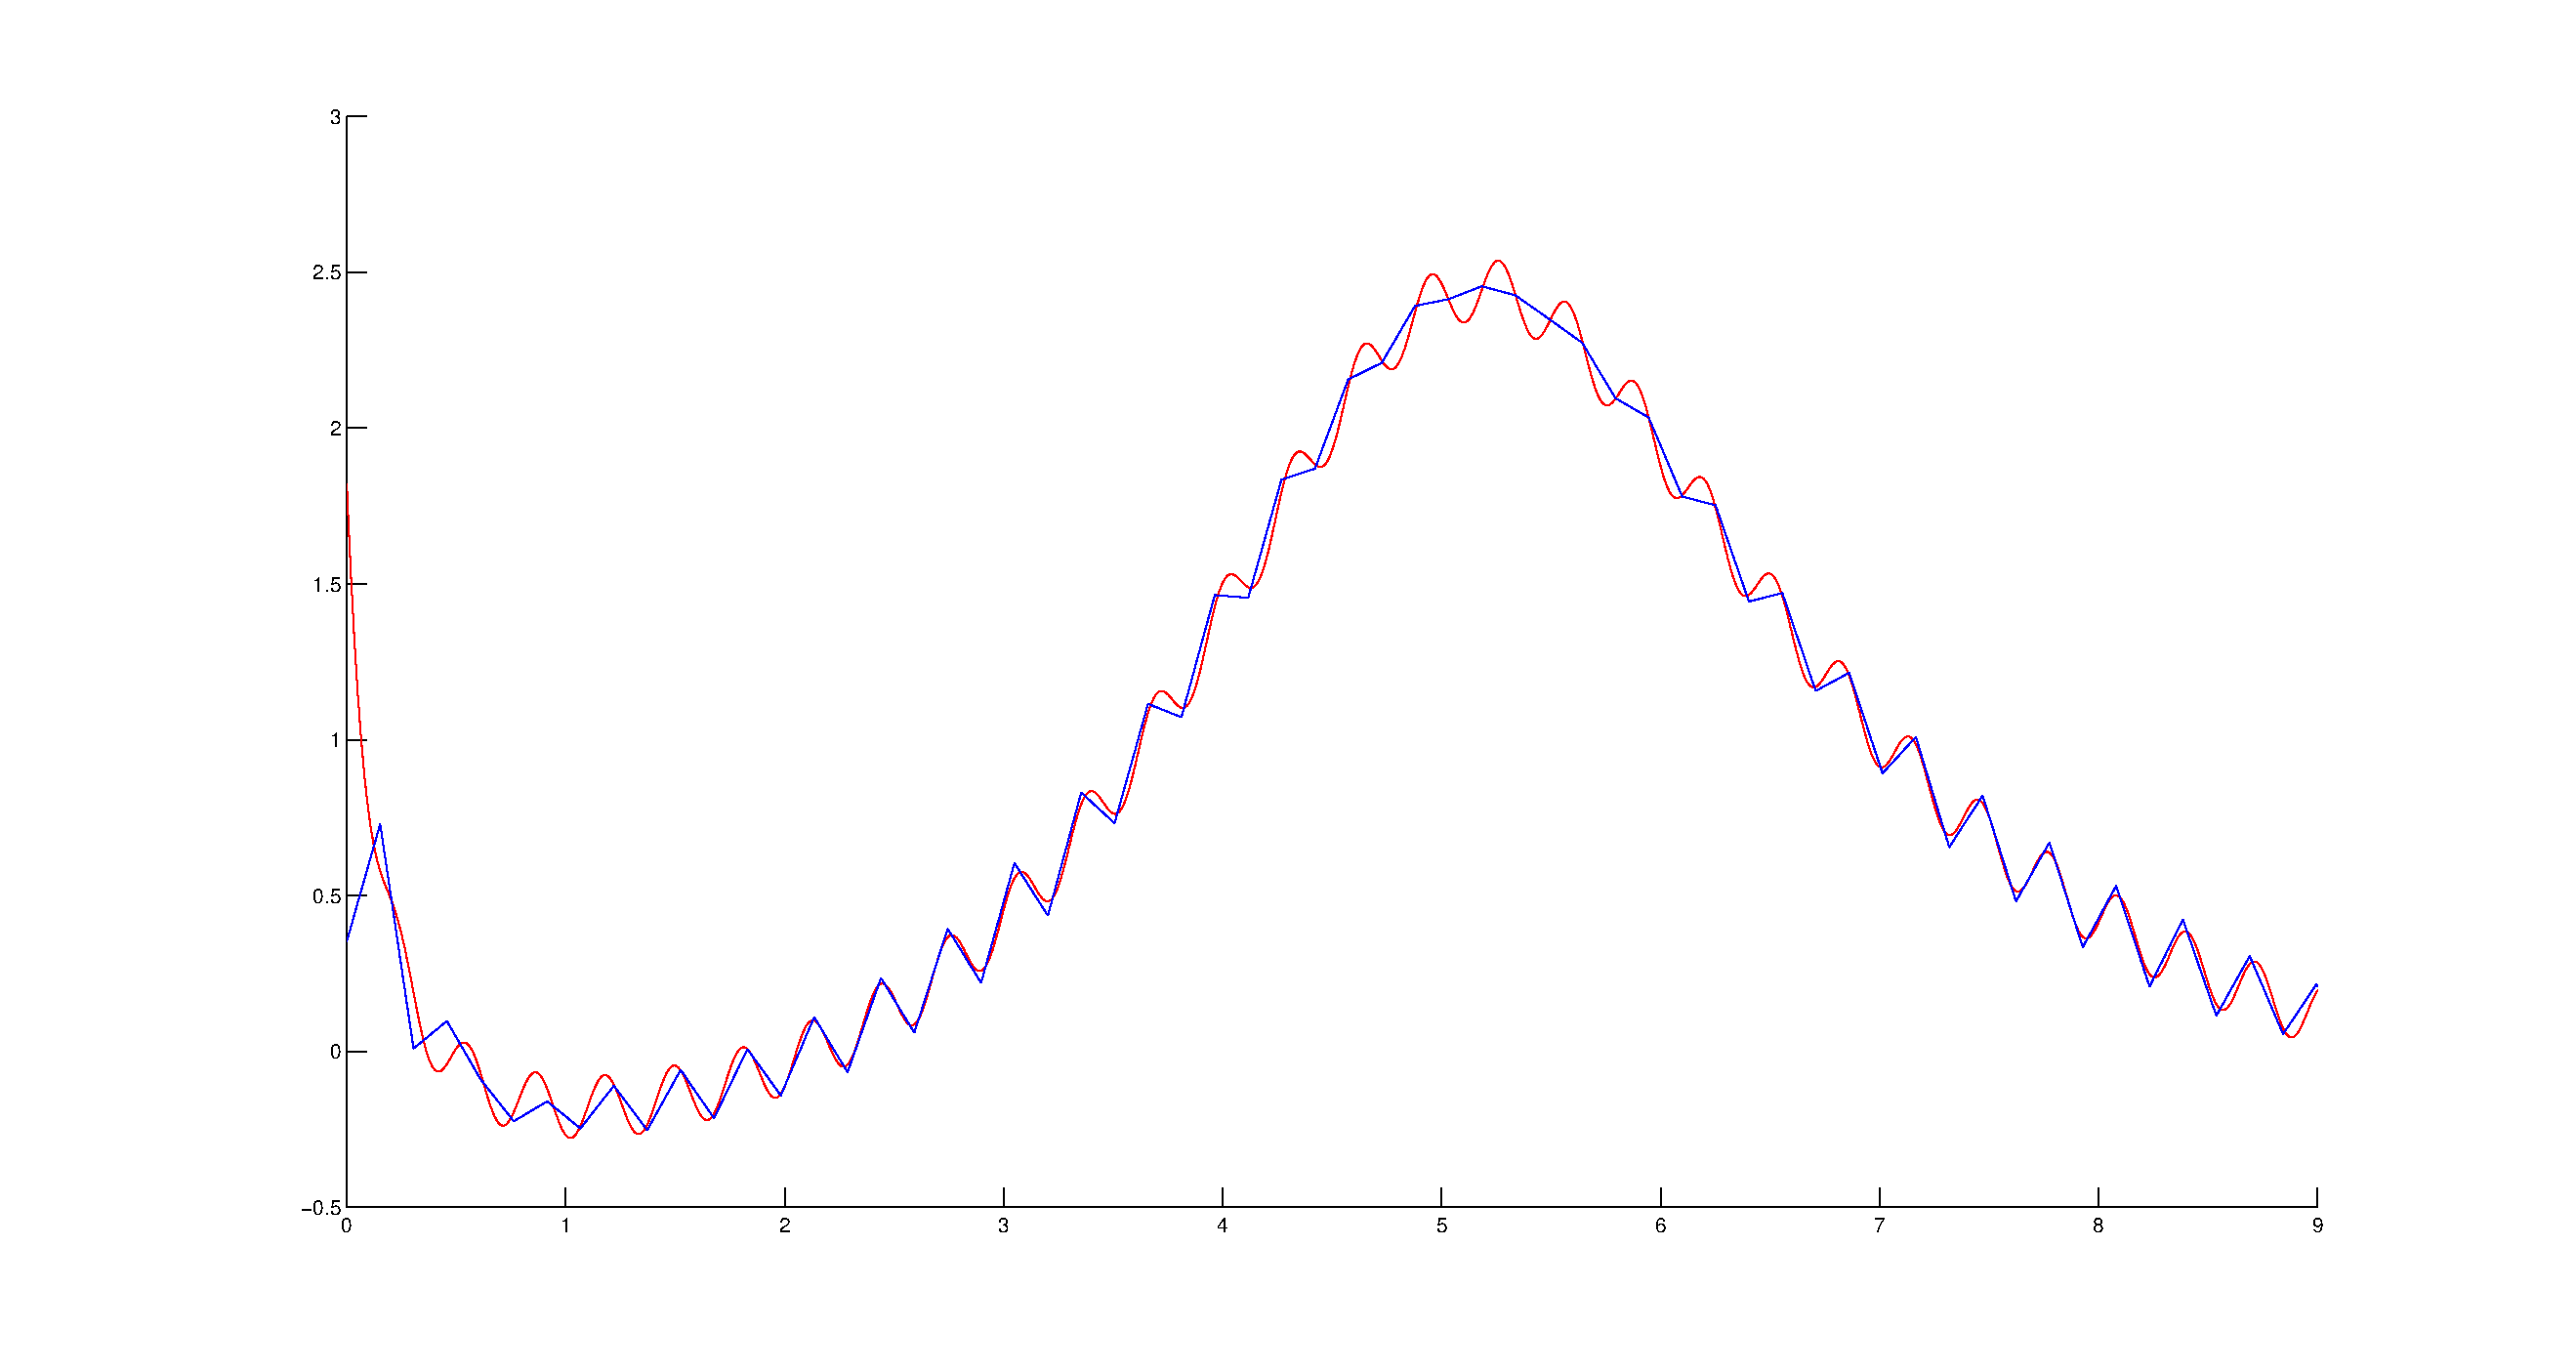
\includegraphics[width=0.55\textwidth]{figfun640agents}\hspace{-0.9cm}
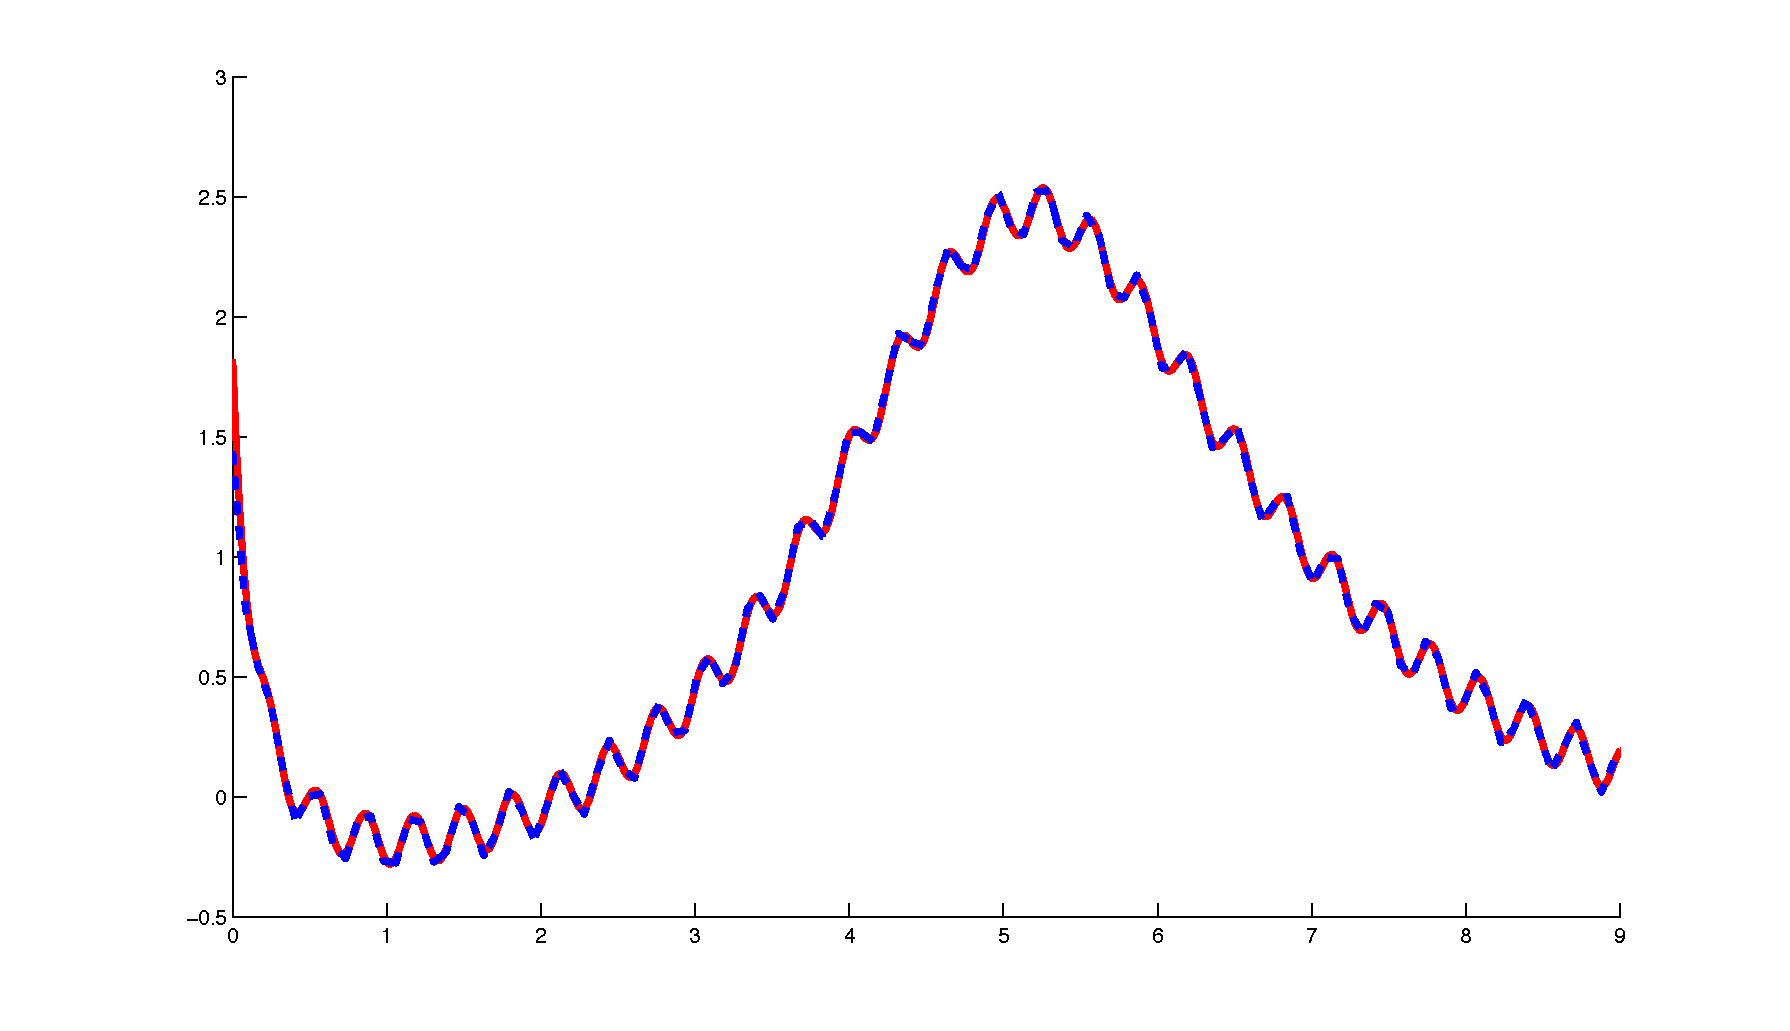
\includegraphics[width=0.55\textwidth]{figfun680agents}
\end{center}
\caption{Iterative reconstruction of a potential with a singularity at the origin and highly oscillatory behavior. In red: the unknown kernel. In blue: its reconstruction by minimization of $\mathcal{E}^{[a],N}$. From left-top to right-bottom: reconstruction with $N = 10, 20, 40, 80$ agents.}\label{variableN2}
\end{figure}

\subsection{Numerical validation of the coercivity condition}\label{numcoer}

We now turn our attention to the coercivity constant $c_T$ appearing in \eqref{eq-coercive} and thoroughly discussed in Section \ref{sec:coerc}. In Figure \ref{errorN} we see a comparison between the evolution of the value of the error functional $\mathcal{E}^{[a],N}_\Delta(\widehat{a}_N)$ and of the $L_2(\R_+,\rho^N)$-error $\|a-\widehat{a}_N\|^2_{L_2(\R_+,\rho^N)}$ for different values of $N$. 

\begin{figure}[h]
\hspace{-1.2cm}
\begin{minipage}{0.58\textwidth}
\begin{center}
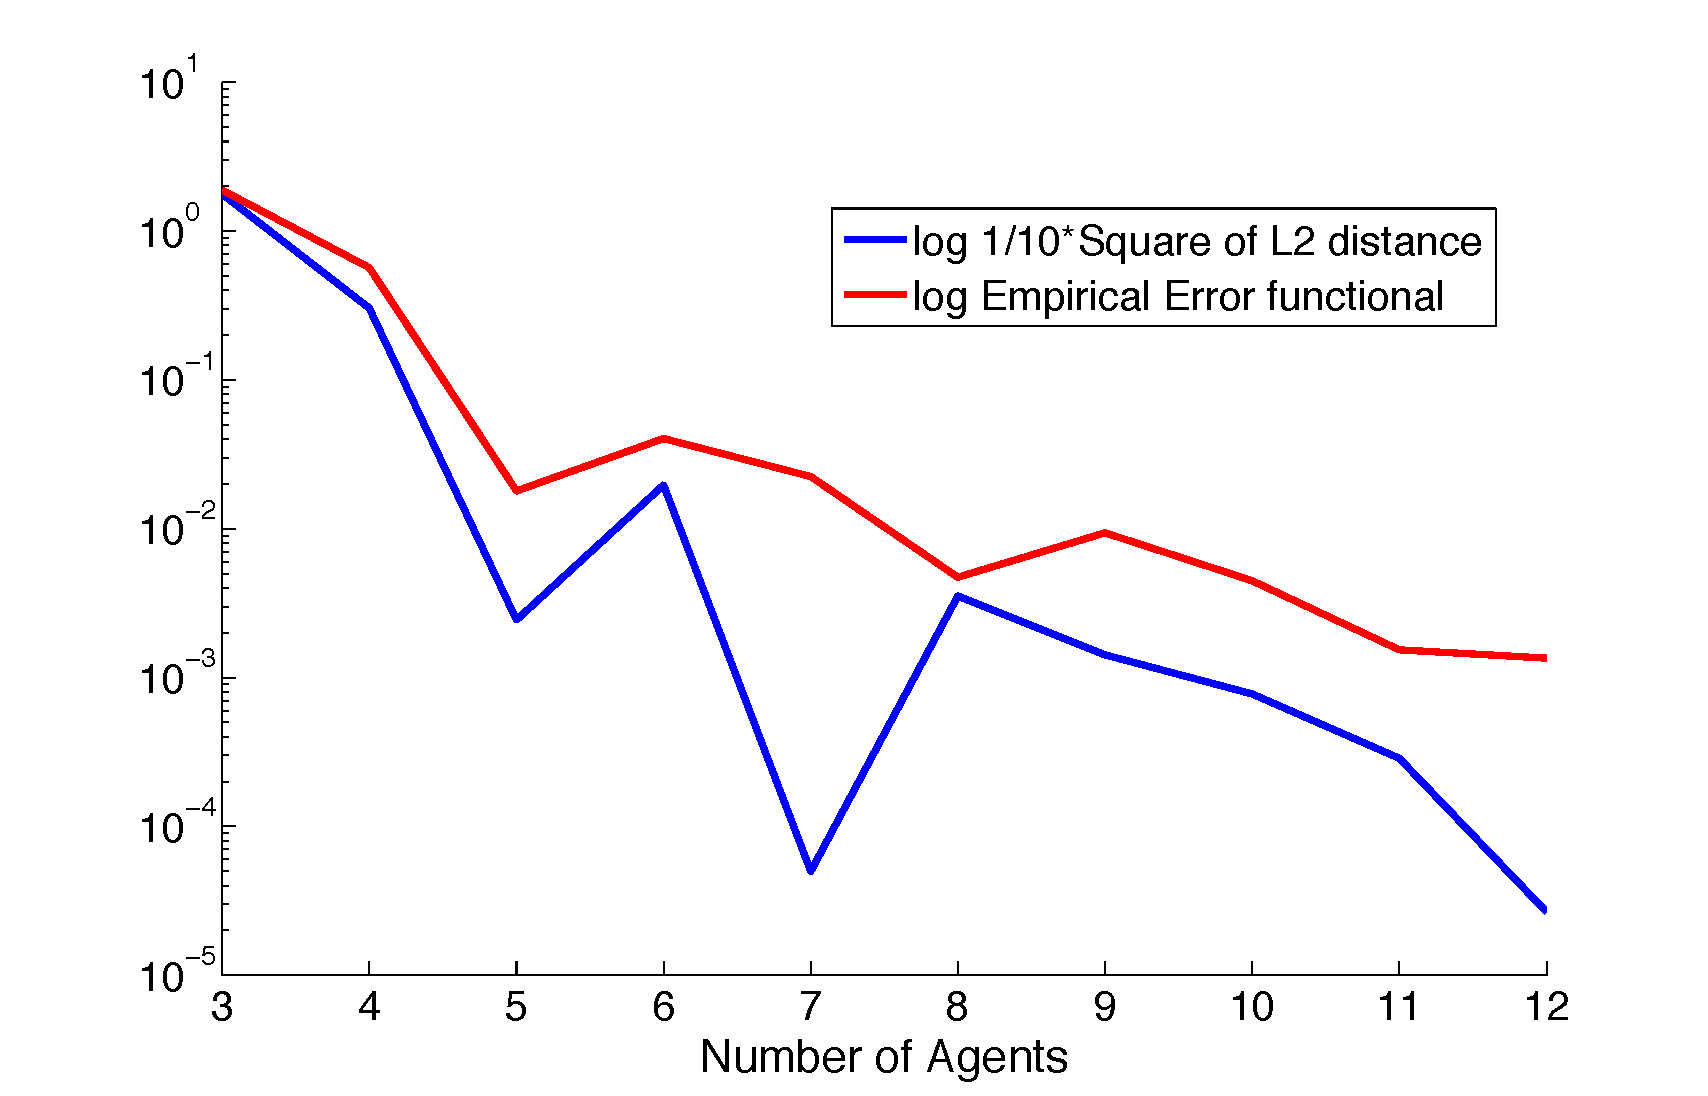
\includegraphics[width=1\textwidth]{fig61l10E2vsENlog}
\end{center}
\label{fig:coerc}
\caption{Plot in logarithmic scale of $\mathcal{E}^{[a],N}(\widehat{a}_N)$ and $\frac{1}{10}\|a-\widehat{a}_N\|^2_{L_2(\R_+,\rho^N)}$ for different values of $N$. In this experiment, we can estimate the constant $c_T$ with the value $\frac{1}{10}$.}\label{errorN}
\end{minipage}
\hspace{0.4cm}
\begin{minipage}{0.55\textwidth}
\begin{center}
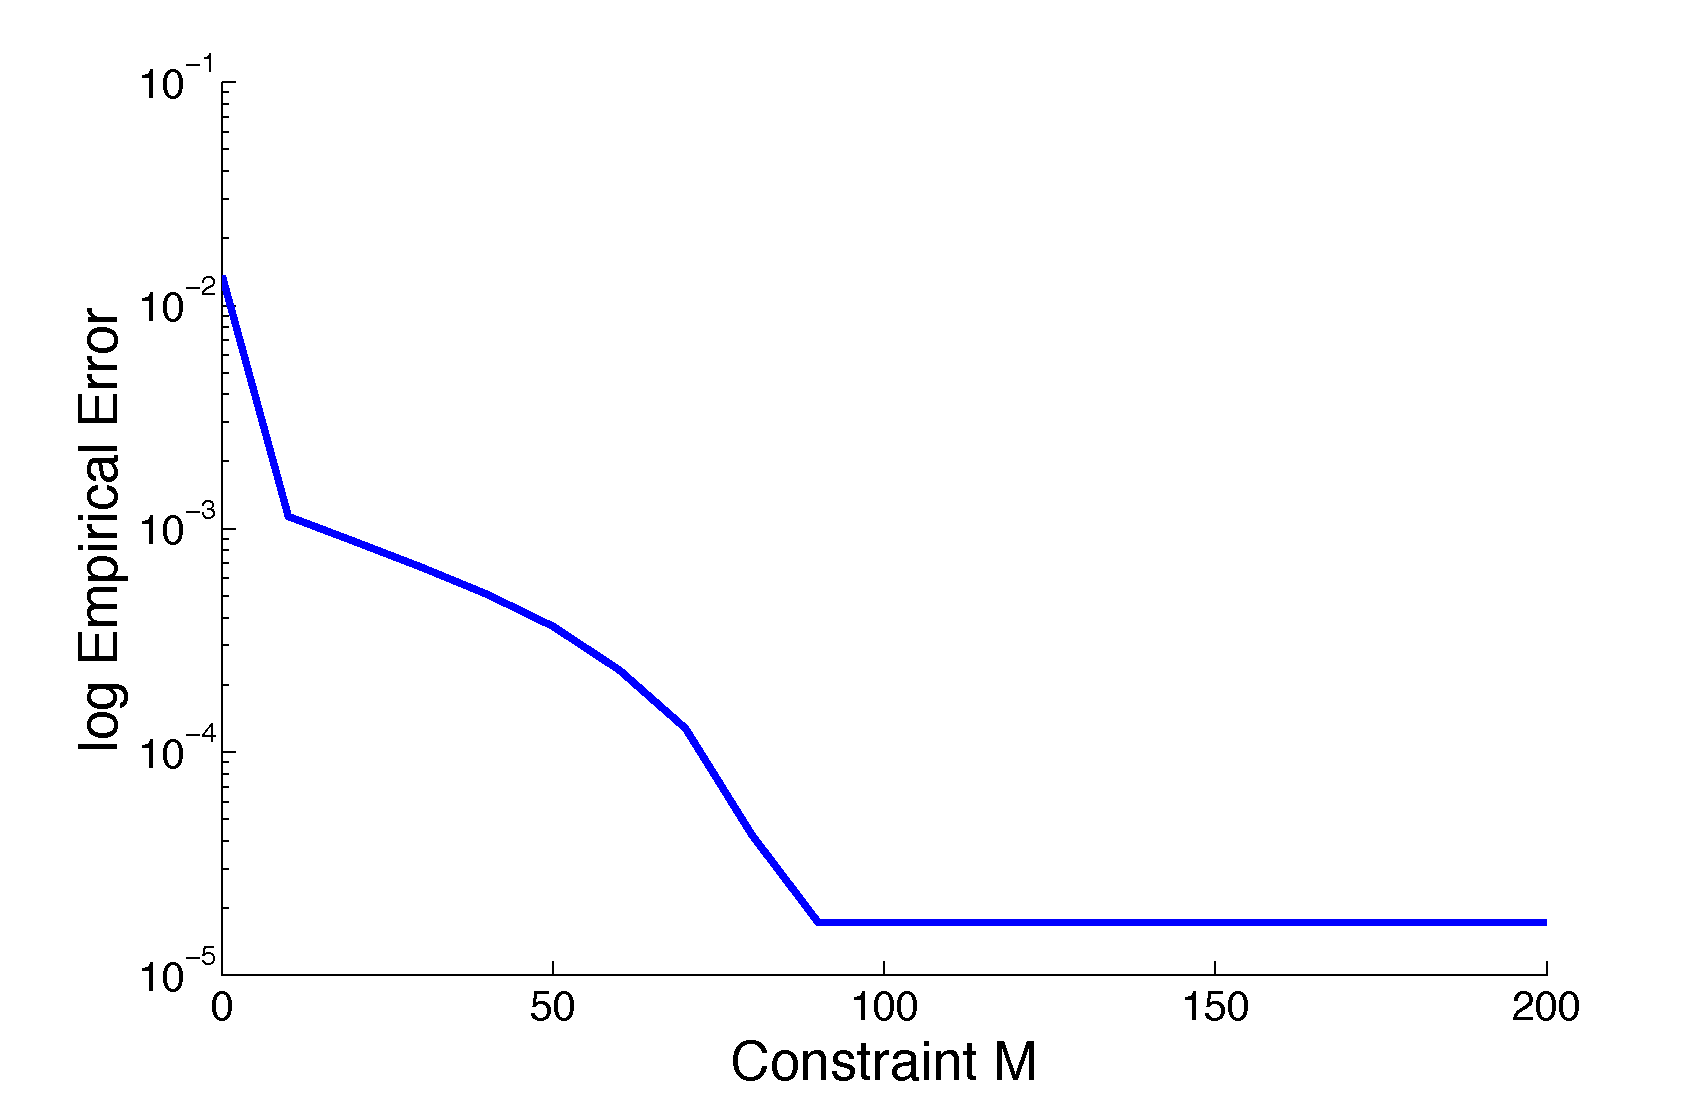
\includegraphics[width=1\textwidth]{figureM2log}
\end{center}
\label{fig:coerc2}
\caption{Values in logarithmic scale of $\mathcal{E}^{[a],N}_\Delta(\widehat a_{N,M})$ for fixed $N = 50$ for different values of $M \in [0,200]$.}\label{Mconstr}
\end{minipage}
\end{figure}

In this experiment, the potential $a$ to be retrieved is the truncated Lennard-Jones type interaction kernel of Figure \ref{variableN} and the parameters used in the algorithm are reported in Table \ref{tab:fig3}.

\begin{table}[h]
\begin{center}
\begin{tabular}{ |c|c|c|c|c|c| }
\hline
  $d$ & $L$ & $T$ & $M$ & $N$ & $D(N)$ \\
\hline
\hline
  $2$ & $5$ & $0.5$ & $100$ & $[3,4,\ldots,12]$ & $3N-5$ \\
\hline
\end{tabular}
\end{center}
\vspace{-0.5cm}
\caption{Parameter values for Figure \ref{errorN}.} \label{tab:fig3} 
\end{table}

For every value of $N$, we have obtained the minimizer $\widehat{a}_N$ of problem \eqref{problem2} and we have computed the errors $\mathcal{E}^{[a],N}(\widehat{a}_N)$ and $\|a-\widehat{a}_N\|^2_{L_2(\R_+,\rho^N)}$. The $L_2(\R_+,\rho^N)$-error multiplied by a factor $\frac{1}{10}$ lies entirely below the curve of $\mathcal{E}^{[a],N}(\widehat{a}_N)$, which let us empirically estimate the value of $c_T$ around that value (see Figures \ref{fig:coerc} and \ref{fig:coerc2}).
%
%The major issue with this experiment is that the minimization procedure quickly reaches values near machine precision. This causes the inability of the approximation to comply with the increasing number of distances explored by the increasing number of agents, and leads to a resurgence of the $L_2(\R_+,\rho^N)$-error, which is defined as
%\begin{align}
%	\|\widehat a-a\|^2_{L_2(\R_+,\rho^N)} = \frac{1}{T}\int_0^T\int_{\R_+}\bigl|\widehat a(s)-a(s)\bigr|^2 s^2 d\varrho^N(t)(s) dt,
%\end{align}
%where $\varrho^N = d_\# \mu^N \otimes \mu^N$.
%Hence, rather than seeing a smooth descent to zero for higher values of $N$, due to finite precision a saw-like pattern emerges. \MMcomment{I do not understand this explanation - you are clearly seeing something I don't see. Which seesaw patterns? In figure \ref{fig:coerc}? Could this be overfitting $D(N)$  not optimal as a function of $N$ and the number of distances explored?}
%%Hence, rather than seeing a smooth descent to zero for higher values of $N$, a saw-like pattern emerges due to the approximation not being able to cope with the increasing number of distances explored (by the increasing number of agents) in the interval $[0,R]$.

\subsection{Tuning the constraint $M$}

Figure \ref{Mconstr1} shows what happens when we modify the value of $M$ in problem \eqref{problem2}. More specifically, we generate $\mu^N_0$ as explained in Section \ref{numfram} once, and we simulate the system starting from $\mu^N_0$ until time $T$. With the data of this single evolution, we solve problem \eqref{problem2} for several values of $M$ and we denote with $\widehat{a}_M \equiv \widehat{a}_{N,M} \equiv \widehat{a}_{N}$ the minimizer obtained with a specific value of $M$. On the left side of Figure \ref{Mconstr1} we show how the reconstruction $\widehat{a}_M$ gets closer and closer to the true potential $a$ (in white) as $M$ increases, while on the right side we illustrate how the original trajectories (again, in white) used for the inverse problem are approximated better and better by those generated with the computed approximation $\widehat{a}_M$, if we let $M$ grow. Table \ref{tab:figM} reports the values of the parameters of these experiments.

\begin{table}[h]
\begin{center}
\begin{tabular}{ |c|c|c|c|c|c|c| }
\hline
 & $d$ & $L$ & $T$ & $M$ & $N$ & $D(N)$ \\
\hline
\hline
 First row & $2$ & $3$ & $1$ & $2.7 \times [10,15,\ldots,40]$ & $20$ & $60$ \\
\hline
 Second row & $2$ & $3$ & $1$ & $1.25 \times [10,15,\ldots,40]$ & $20$ & $150$ \\
\hline
\end{tabular}
\end{center}
\vspace{-0.5cm}
\caption{Parameter values for Figure \ref{Mconstr1}.} \label{tab:figM} 
\end{table}

\begin{figure}[h!]
\begin{center}
\hspace{-0.7cm}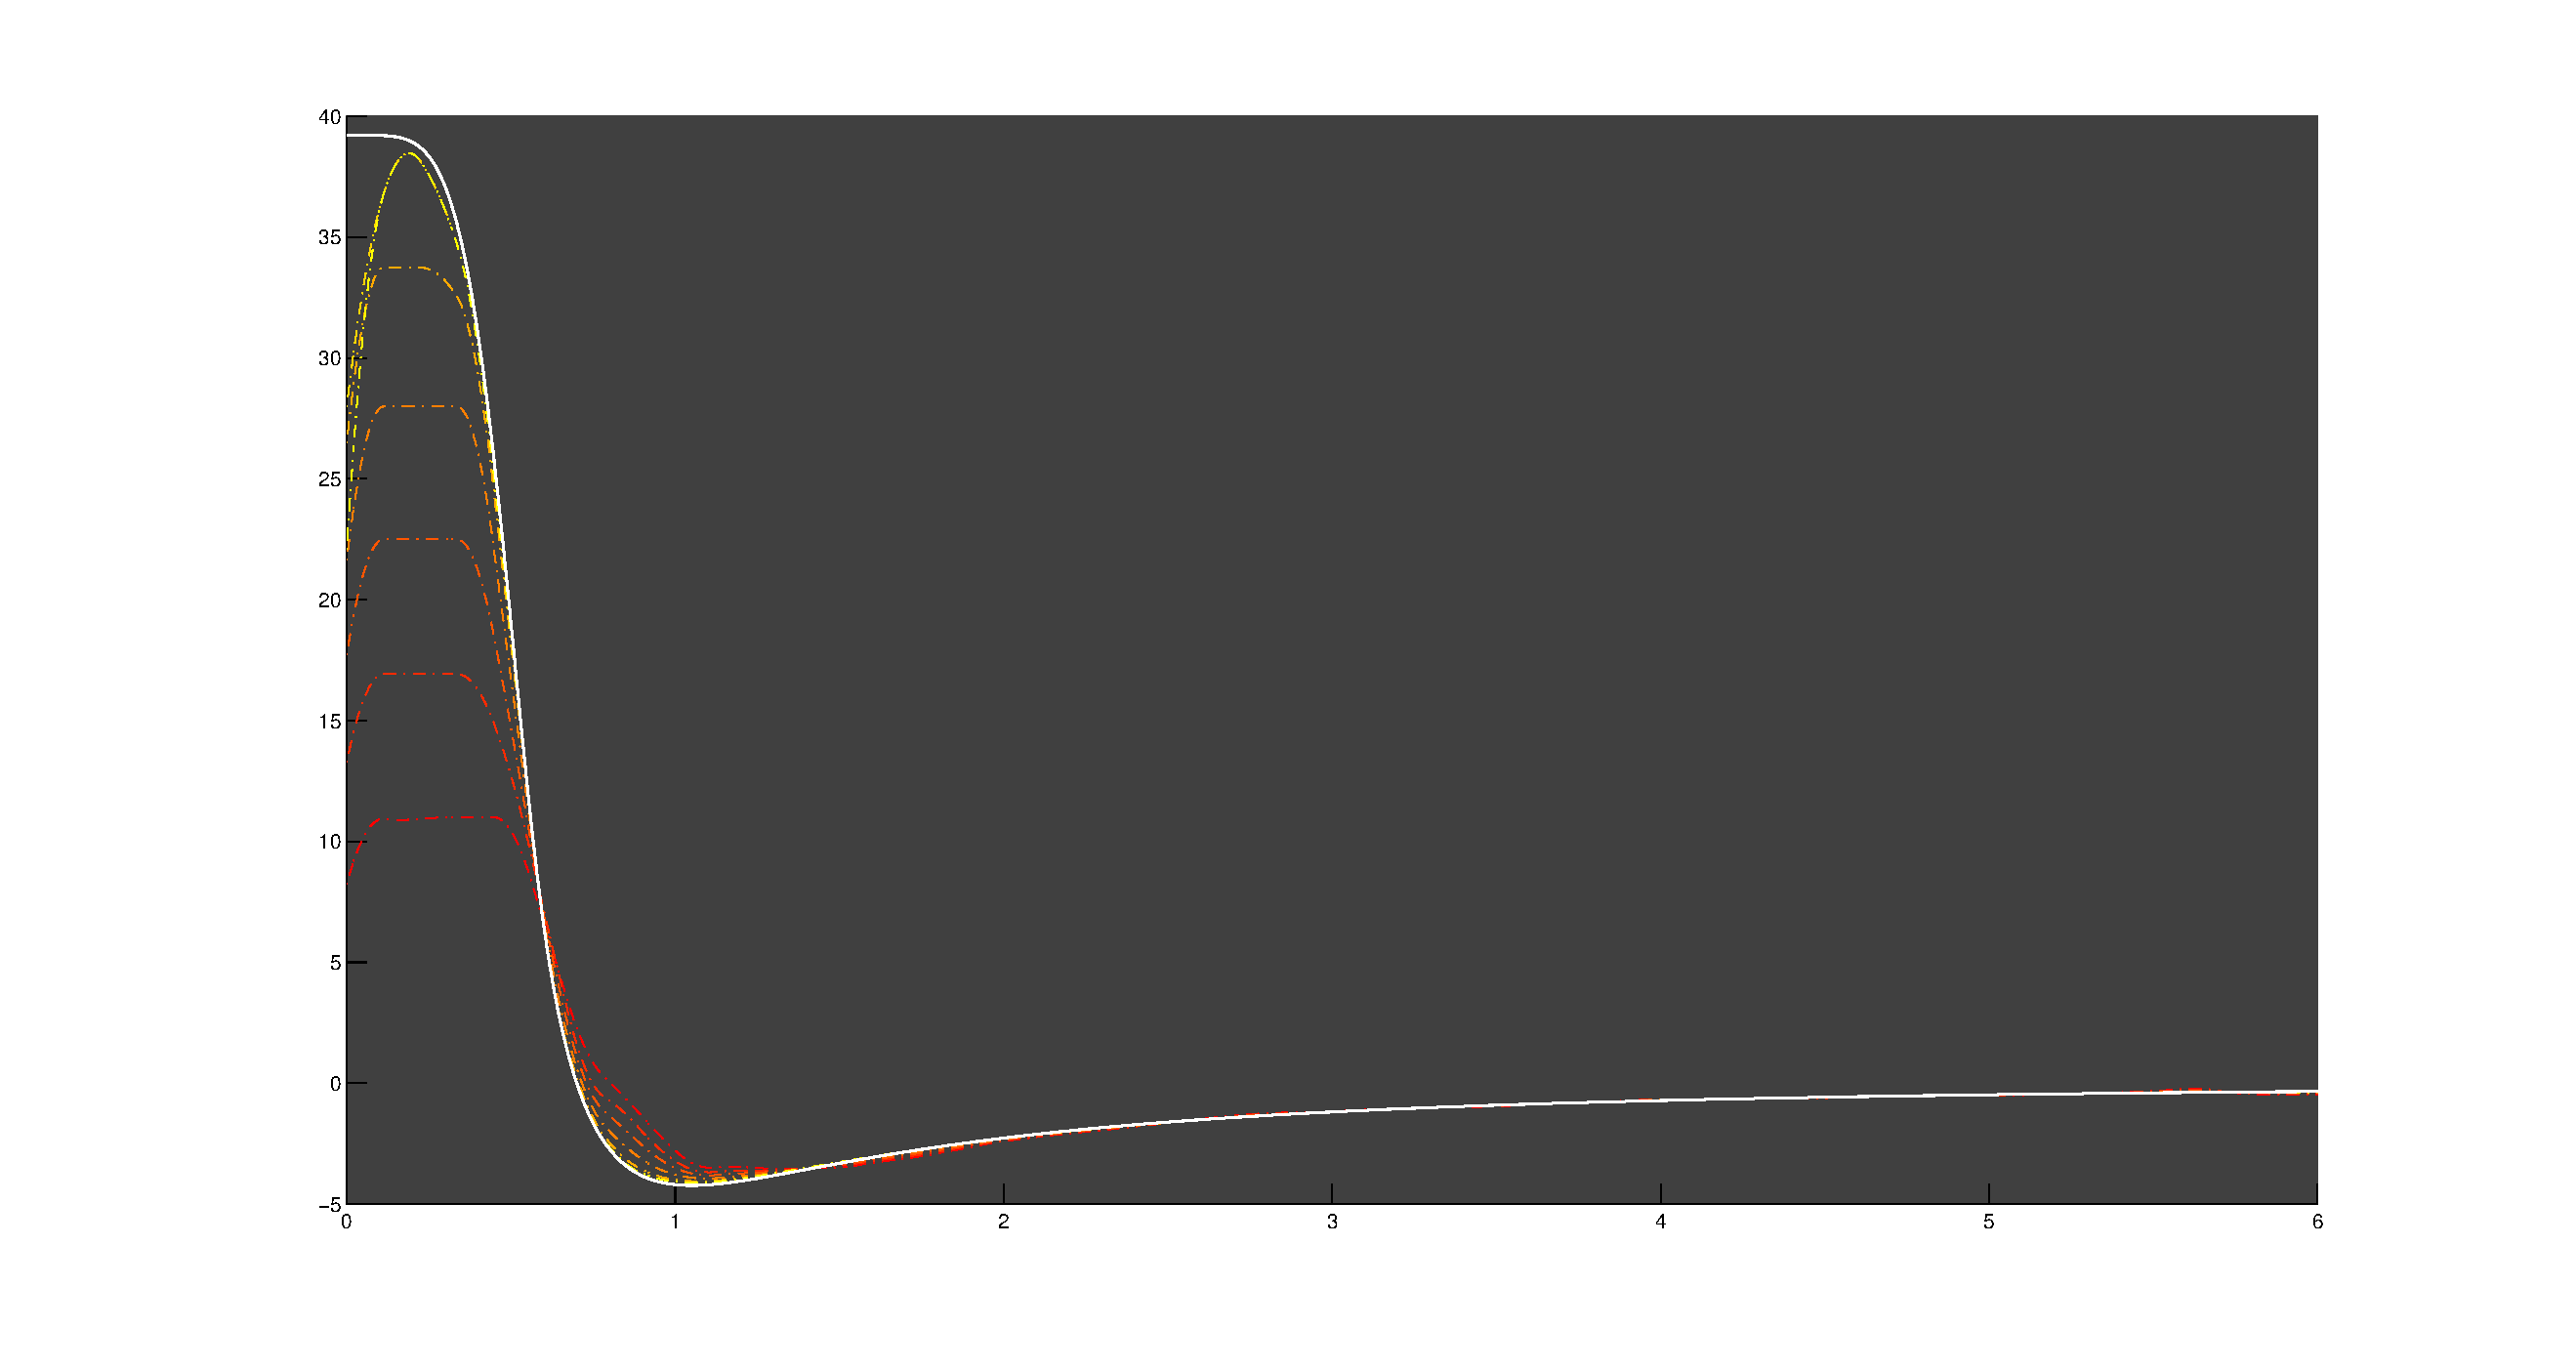
\includegraphics[width=0.625\textwidth]{figPotfun8}\hspace{-0.9cm}
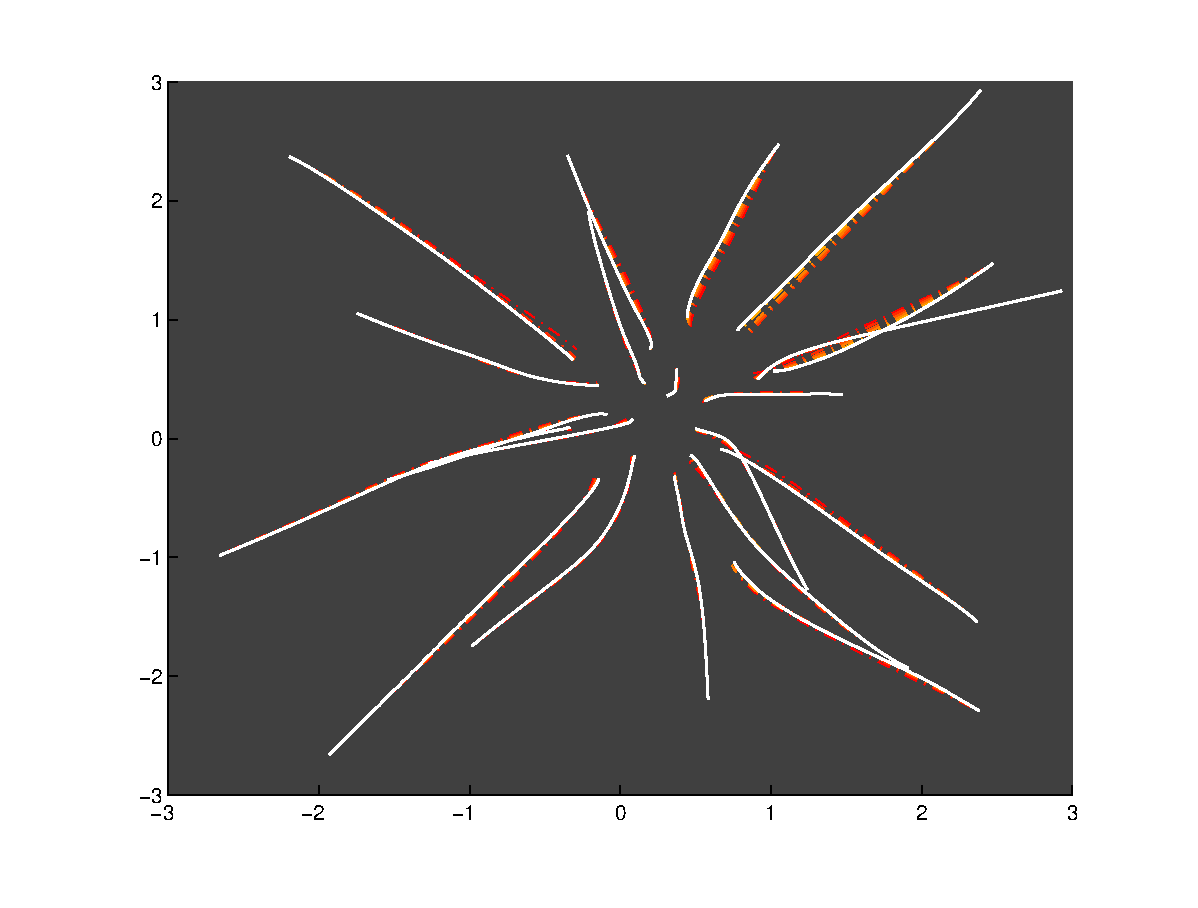
\includegraphics[width=0.475\textwidth]{figTrajfun8}\\
\hspace{-0.7cm}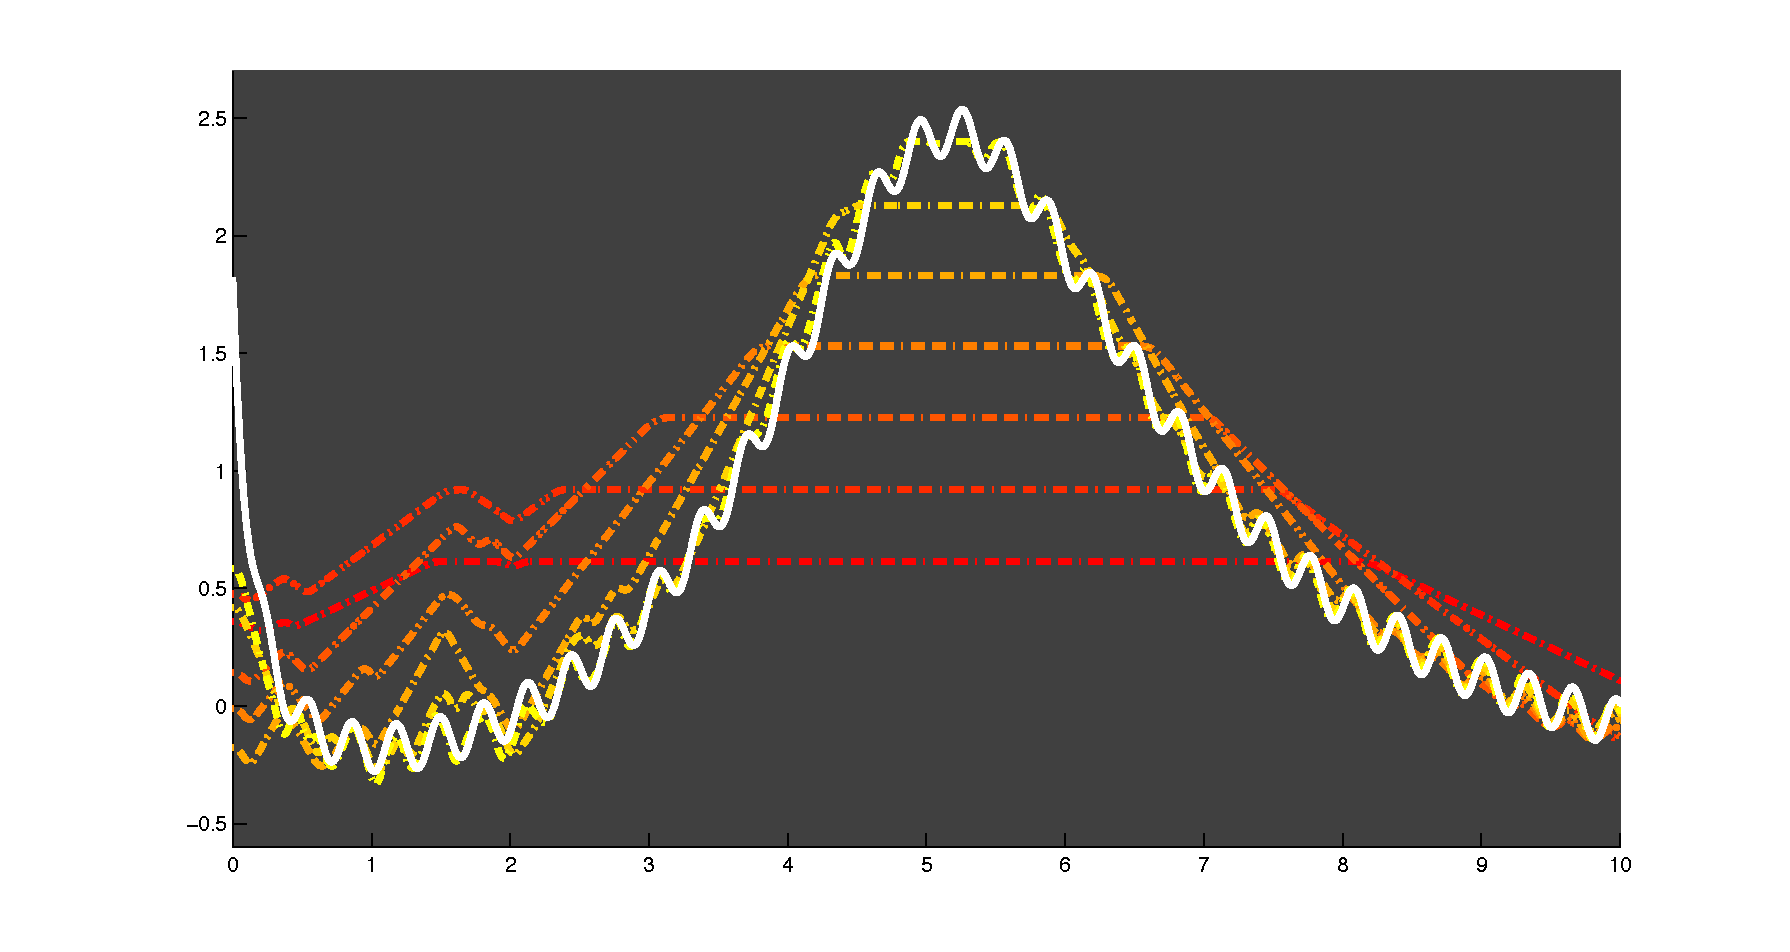
\includegraphics[width=0.645\textwidth]{figPotfun61}\hspace{-0.9cm}
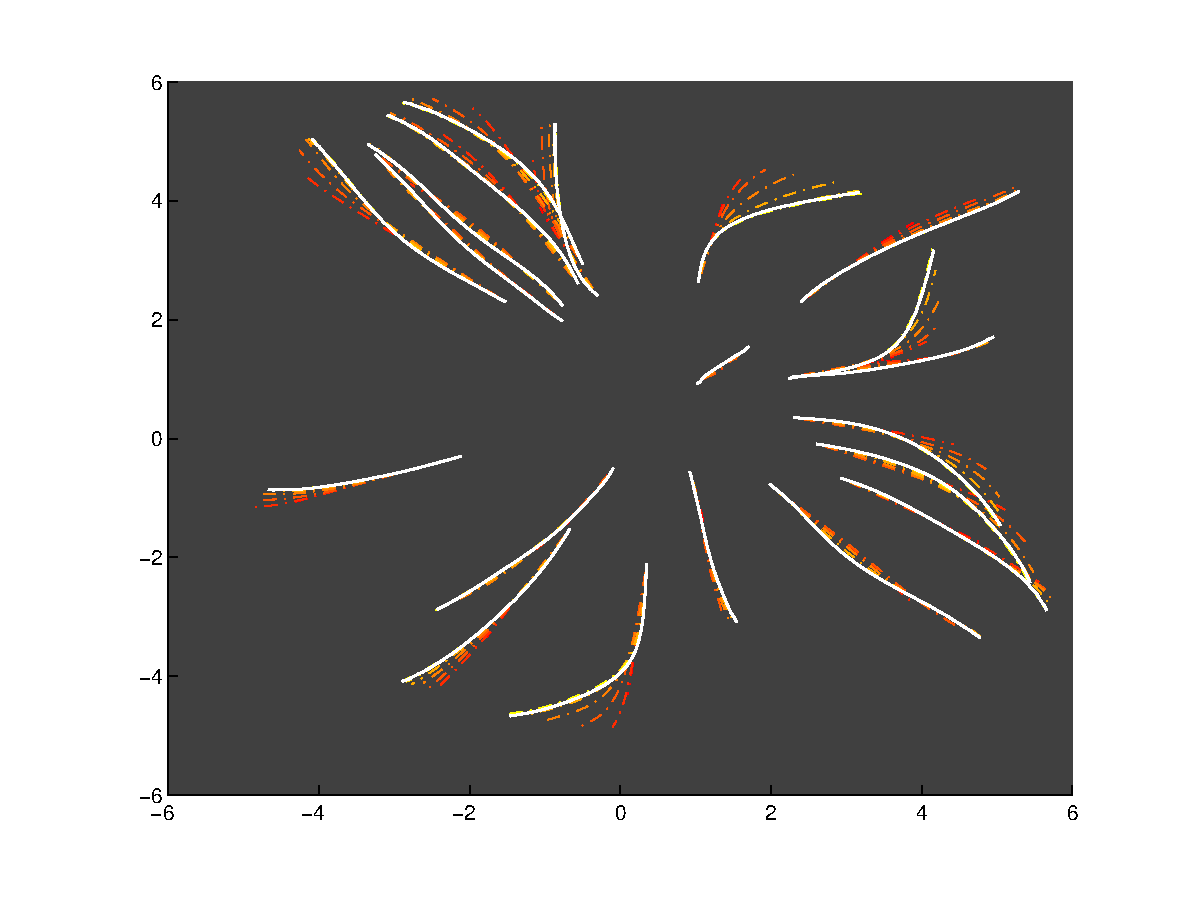
\includegraphics[width=0.455\textwidth]{figTrajfun61}
\end{center}
\caption{Different reconstructions of a potential for different values of $M$. On the left column: the true kernel in white and its reconstructions for different $M$; the brighter the curve, the larger the $M$. On the right column: the true trajectories of the agents in white, the trajectories associated to the reconstructed potentials with the same color.}\label{Mconstr1}
\end{figure}

So far we have no  {\it a priori} criteria to sieve those values of $M$, which enable a successful reconstruction of a potential $a \in X$. However,  the tuning {\it a posteriori} of the parameter $M>0$ turns out to be rather easy. In fact, for $N$ fixed the minimizers $\widehat a_{N,M}$ have the property that the map
$$
 M \mapsto   \mathcal E^{[a],N}(\widehat a_{N,M})
$$
is monotonically decreasing as a function of the constraint parameter $M$ and it becomes constant for $M\geq M^*$, for $M^*>0$ which, as shown empirically, does not depend on $N$. This special value $M^*$ is indeed the ``right" parameter for the $L_\infty$ bound. For such a choice, we show that, if we let $N$ grow, the minimizers $\widehat{a}_N$ approximates better and better the unknown potential $a$. 
Figure \ref{Mconstr} documents precisely this expected behavior.

\begin{figure}[h!]
\begin{center}
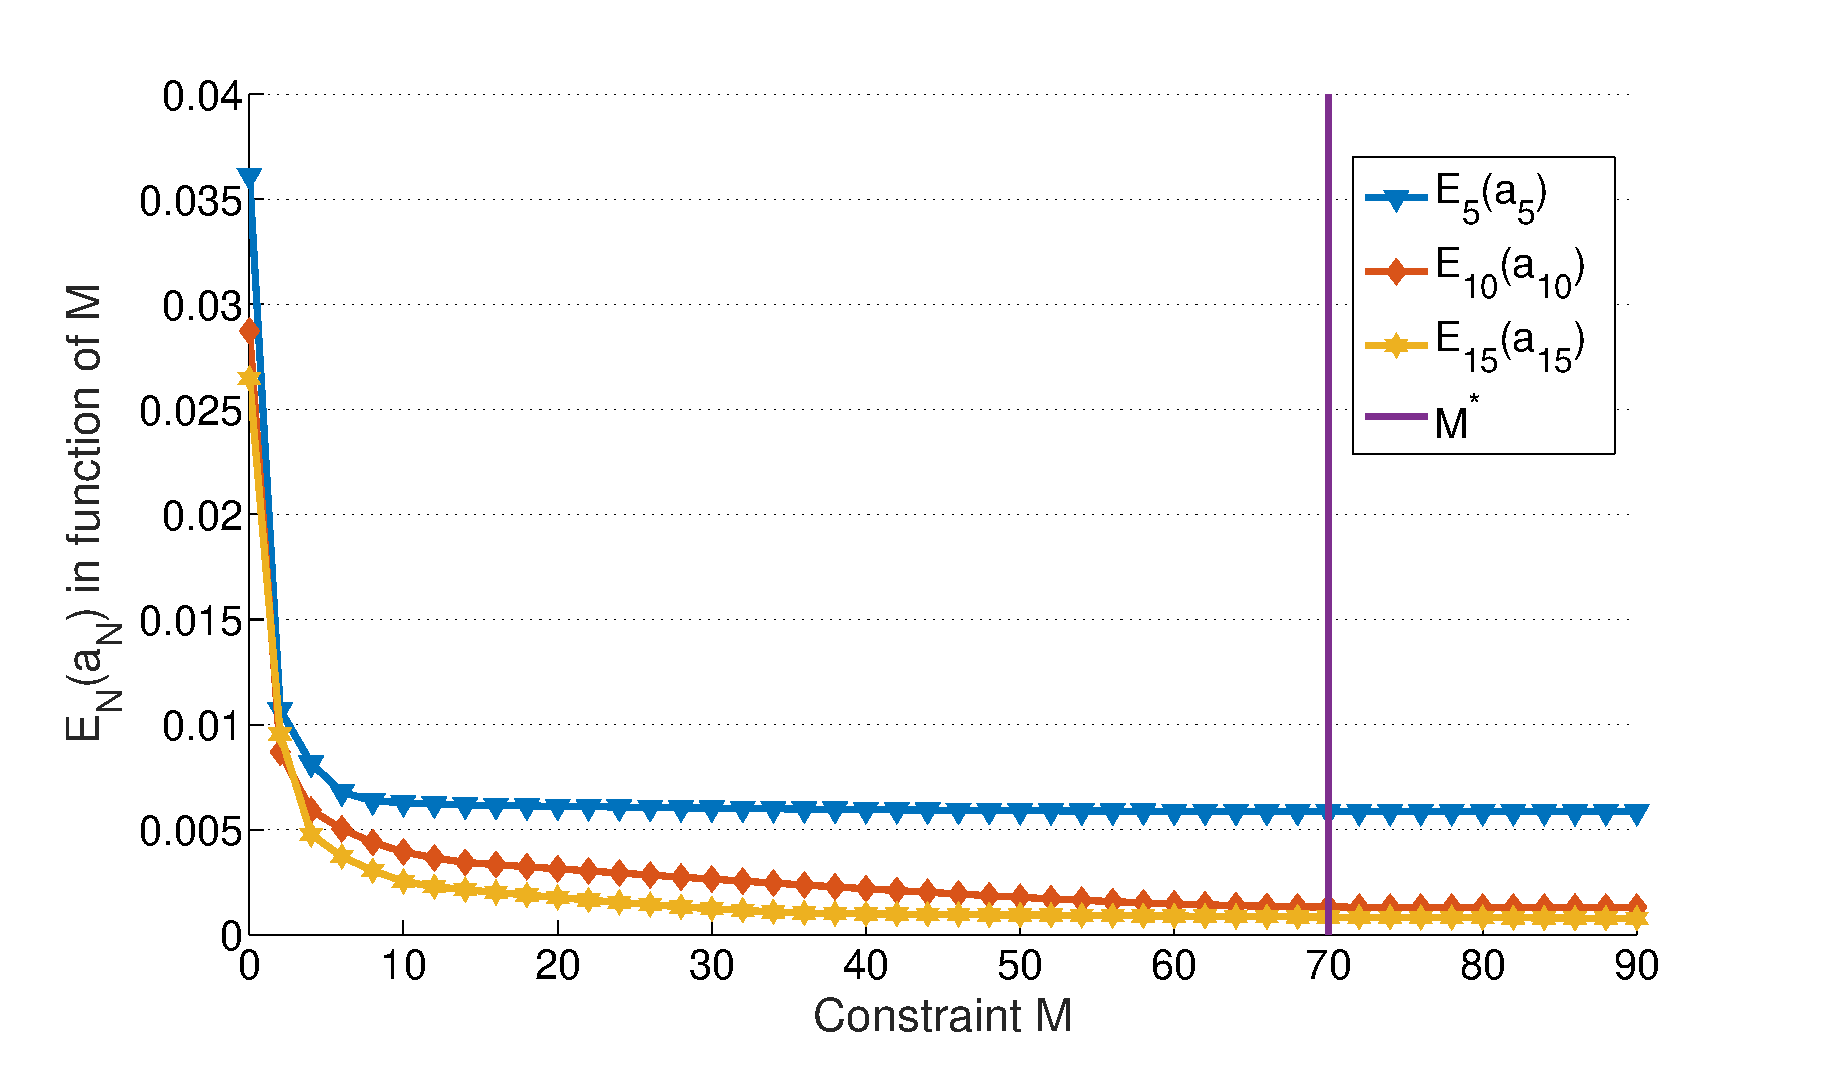
\includegraphics[width=0.8\textwidth]{DifferentM3}
\end{center}
\caption{Behavior of the error $\mathcal E^{[a],N}(\widehat a_{N,M})$ as a function of the constraint $M$ for different values of $N$.}\label{Mconstr}
\end{figure}

\subsection{Montecarlo-like reconstructions for $N$ fixed}

We mimic now the  mean-field reconstruction strategy, by multiple randomized draw of $N$ particles as initial conditions i.i. distributed according to $\mu_0$ for $N$ fixed and relatively small. Indeed, problem \eqref{problem2} can swiftly become computationally unfeasible when $N$ is moderately large, also because the dimension of the approximating subspaces $V_N$ needs to increase with $N$ too.  We consider, for a fixed $N$, several discrete initial data $(\mu^N_{0,\theta})_{\theta= 1}^{\Theta}$ all independently drawn from the same distribution $\mu_0$ (in our case, the $d$-dimensional cube $[-L,L]^d$). For every $\theta = 1,\ldots,\Theta$, we simulate the system until time $T$ and, with the trajectories we obtained, we solve problem \eqref{problem2}. At the end of this procedure, we have a family of reconstructed potentials $(\widehat{a}_{N,\theta})_{\theta= 1}^{\Theta}$, all approximating the same true kernel $a$. Empirically averaging these potentials, we obtain an approximation
\begin{align*}
\widehat{a}_N(r) = \frac{1}{\Theta} \sum^{\Theta}_{\theta = 1}\widehat{a}_{N,\theta}(r), \quad \text{ for every } r \in [0,R],
\end{align*}
which we claim to be a better approximation to the true kernel $a$ than any single snapshots. To support this claim, we report in Figure \ref{fixedN} the outcome of an experiment whose data can be found in Table \ref{tab:fig5}.

\begin{table}[h]
\begin{center}
\begin{tabular}{ |c|c|c|c|c|c|c| }
\hline
  $d$ & $L$ & $T$ & $M$ & $N$ & $D(N)$ & $\Theta$ \\
\hline
\hline
  $2$ & $2$ & $0.5$ & $1000$ & $50$ & $150$ & 5  \\
\hline
\end{tabular}
\end{center}
\vspace{-0.5cm}
\caption{Parameter values for the experiment of Figure \ref{fixedN}.} \label{tab:fig5} 
\end{table}

\begin{figure}[h!]
\begin{center}
\hspace{-1cm}
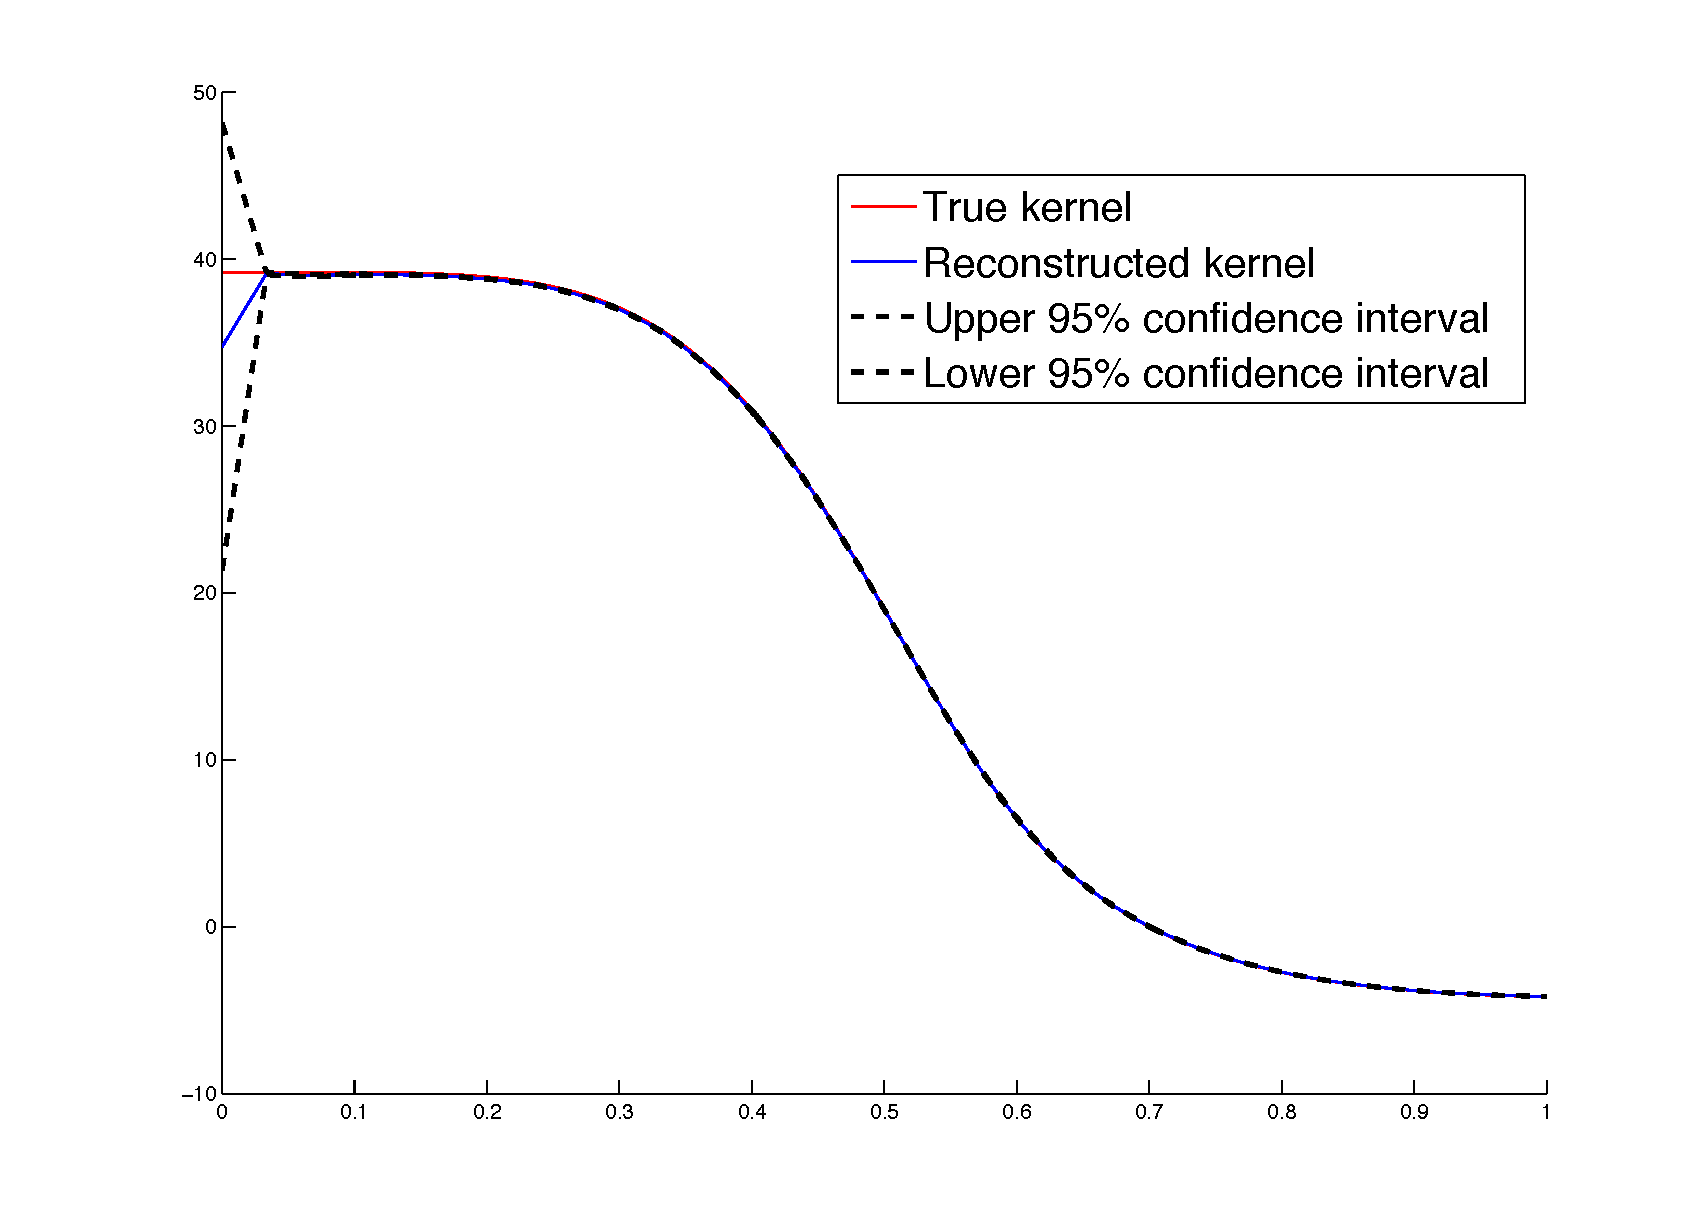
\includegraphics[width=0.56\textwidth]{figNfissofun8alias}\hspace{-0.9cm}
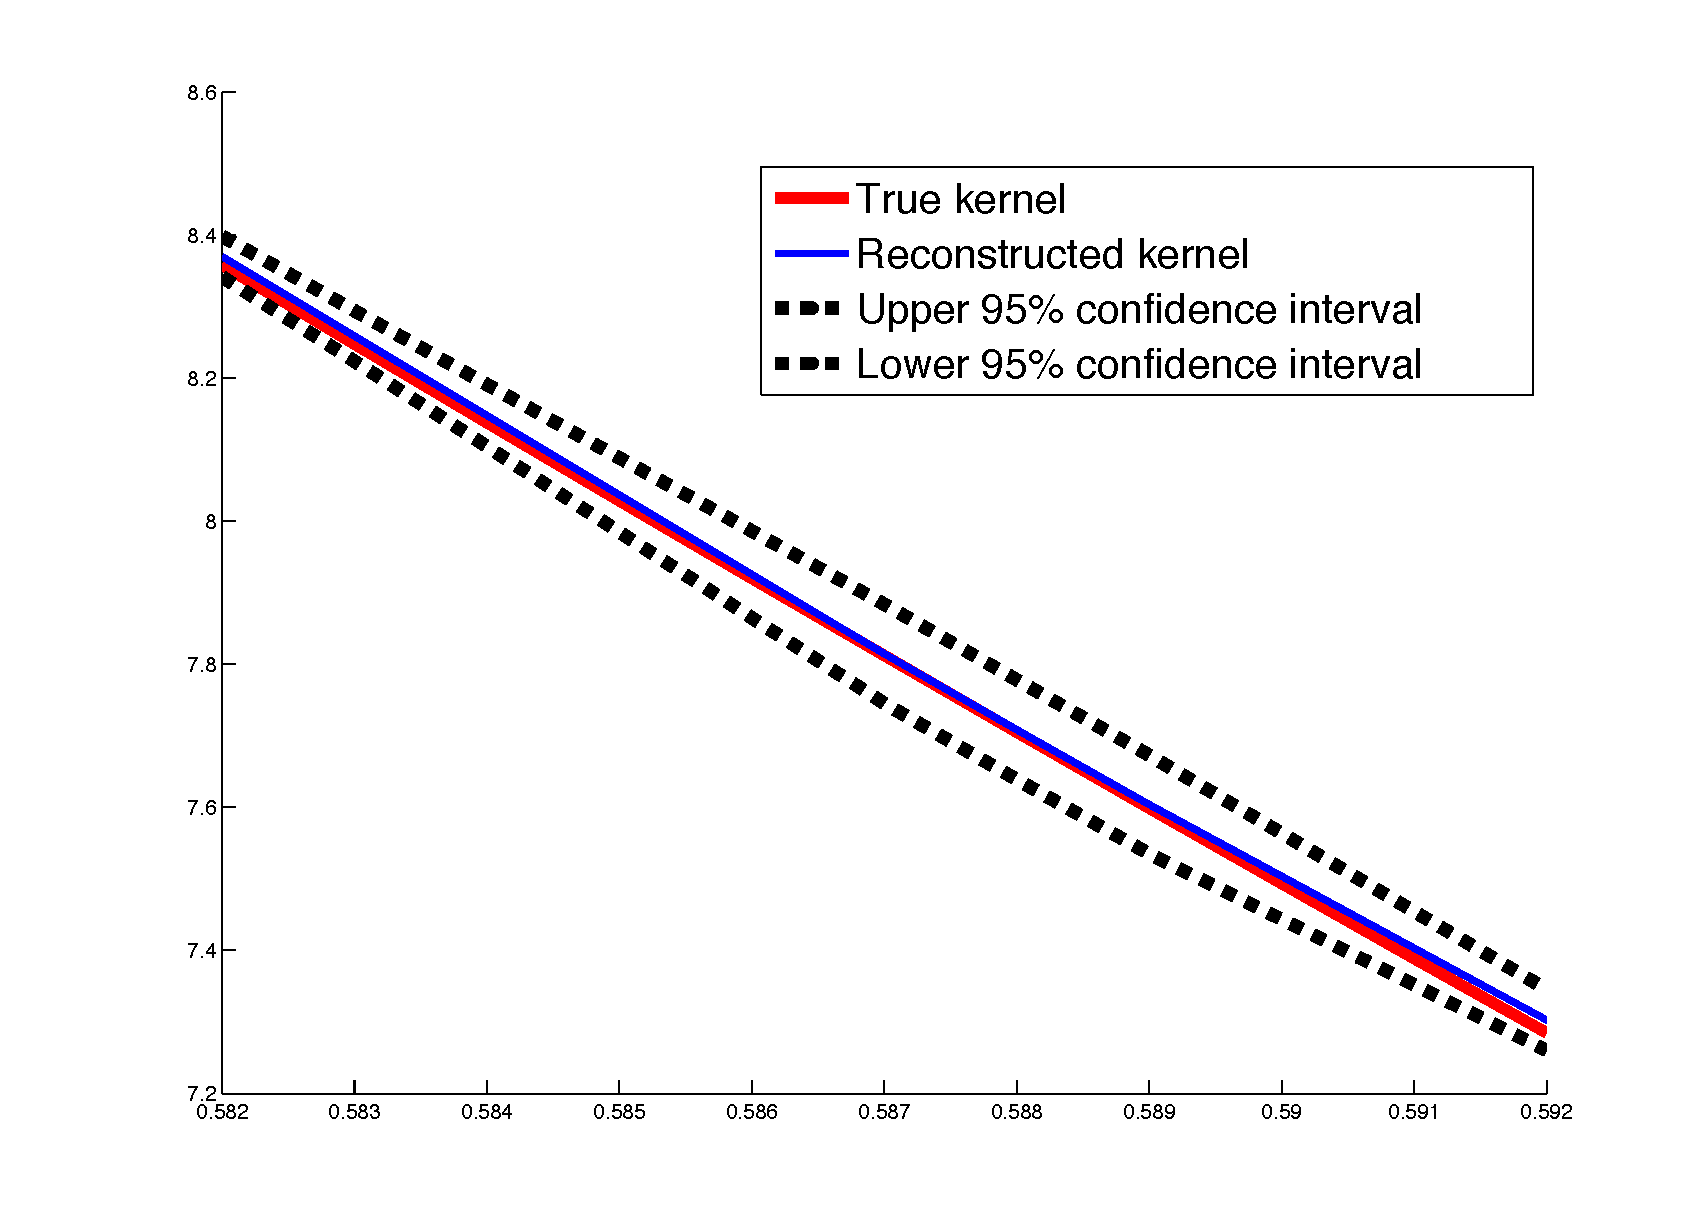
\includegraphics[width=0.55\textwidth]{figNfissofun8part}
\end{center}
\caption{Reconstruction of $a$ obtained by averaging 5 solutions of the minimization of $\mathcal{E}^{[a],N}_\Delta$ for $N = 50$. In red: the unknown kernel. In blue: the average of reconstructions. In black: 95\% confidence interval for the parameter estimates returned by the Matlab function \texttt{normfit}. The figure on the right shows a zoom of the left figure.}\label{fixedN}
\end{figure}